\documentclass[]{article}

\usepackage{graphicx}
\usepackage{amssymb}
\usepackage{amsthm}
\usepackage{amsmath}
\usepackage{multirow}
\usepackage[section]{placeins}
\usepackage{listings}
\usepackage{hyperref}
\hypersetup{
	colorlinks,
	citecolor=black
	filecolor=black,
	linkcolor=blue,
	urlcolor=black
}
\lstset{
	language=MATLAB,
	basicstyle=\scriptsize\sffamily,
	numbers=left,
	numberstyle=\tiny,
	frame=tb,
	columns=fullflexible,
	showstringspaces=false
}

%opening
\title{EML6934 Optimal Control \\ Final Project}
\author{Elias Reyes}

\begin{document}
	
	\maketitle
	\thispagestyle{empty}
	\newpage
	\pagenumbering{roman}
	\newpage
	\tableofcontents
	\newpage
	\listoffigures
	\listoftables
	\newpage
	\lstlistoflistings
	\newpage
	\pagenumbering{arabic}
	
	\section{Problem Statement}
	\section{Differential Equations of Motion}
	The differential equations of motion were derived using both Newton's second law. The schematic for the problem can be seen Figure \ref{fig:schematic}. The spacecraft is modeled as point \(P\) of  mass \(m\). The spacecraft moves relative to an inertial reference frame \(l\). The reference frame fixed in \(l\) is expressed as \(\{e_{x},e_{y},e_{z}\}\). The position of the spacecraft is denoted as \(r_{P/O}\), where \(O\) is modeled as the sun, fixed in \(l\). The spacecraft is parameterized in the basis \(\{u_{r},u_{\theta},u_{z}\}\), where the rotation is about \(u_{z}\) = \(e_{z}\). The rotation creates an angle \(\theta\) between \(e_{x}\) and \(u_{r}\), which can be seen in Figure \ref{fig:rotation2}.
	\begin{figure}
		\centering
		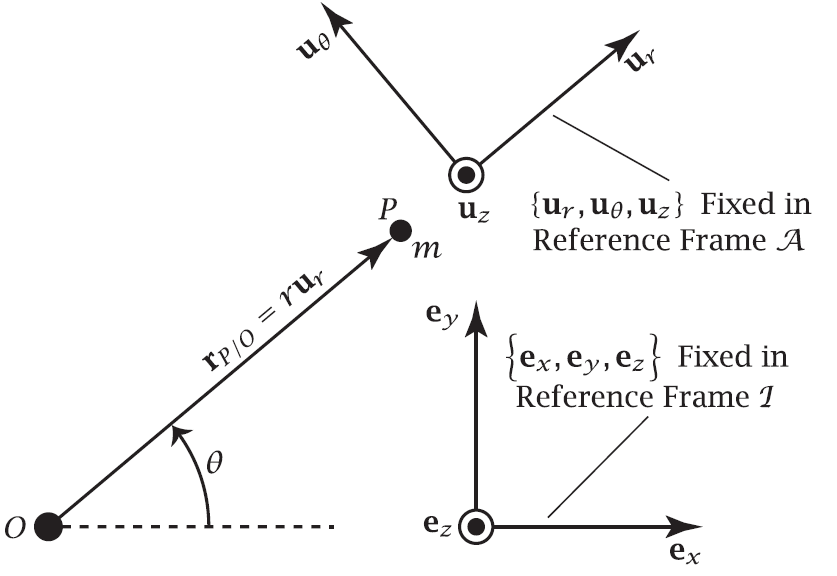
\includegraphics[width=85mm,scale=0.85]{midterm_schematic.png}
		\caption{Schematic of particle moving in an inertially fixed plane}
		\label{fig:schematic}
	\end{figure}
	\begin{figure}
		\centering
		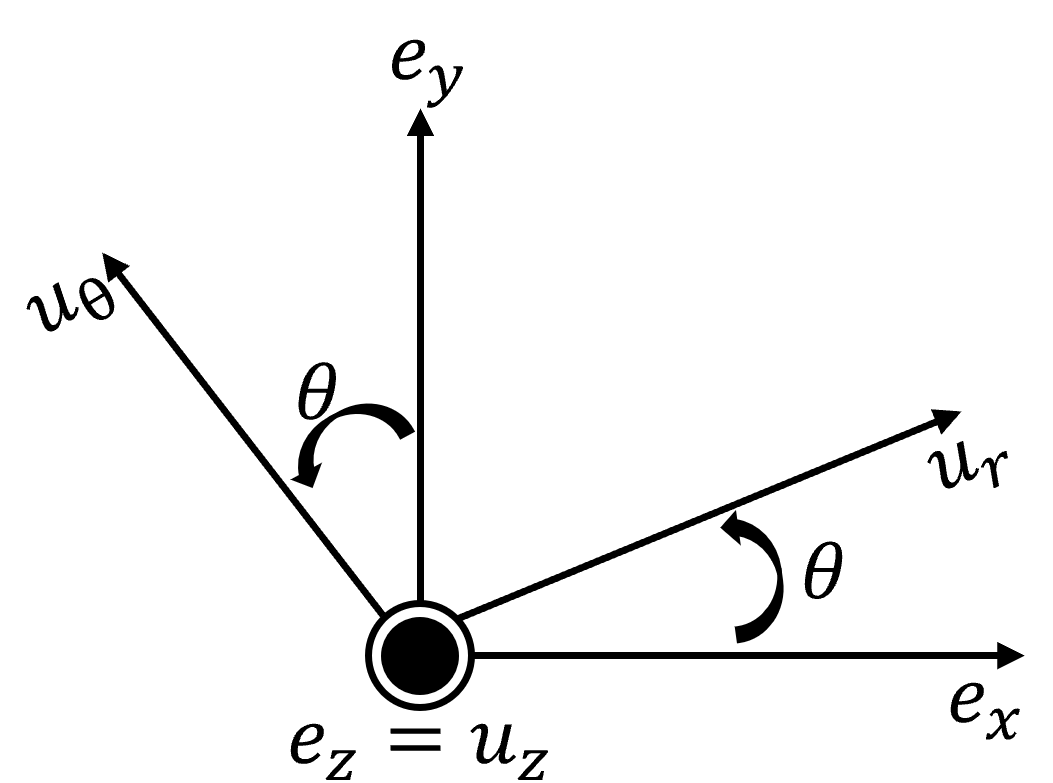
\includegraphics[width=75mm,scale=0.75]{rotation.png}
		\caption{Reference frame rotation}
		\label{fig:rotation2}
	\end{figure}
	\noindent 
	Two forces are said to act on the spacecraft. The first is the gravitational force which is given as
	\begin{equation} \label{grav_force}
		G = -m\mu\frac{r_{P/O}}{||r_{P/O}||^3},
	\end{equation}
	%\[G = -m\mu\frac{r_{P/O}}{||r_{P/O}||^3},\]
	while the second is the thrust force given as\\
	\begin{equation} \label{thrust_force}
		T = Tw,
	\end{equation}
	%\[T = Tw,\]
	where \(w\) is the unit vector that lies an angle \(\beta\) from the direction \(u_{\theta}\) as seen in Figure \ref{fig:beta}.
	\begin{figure}
		\centering
		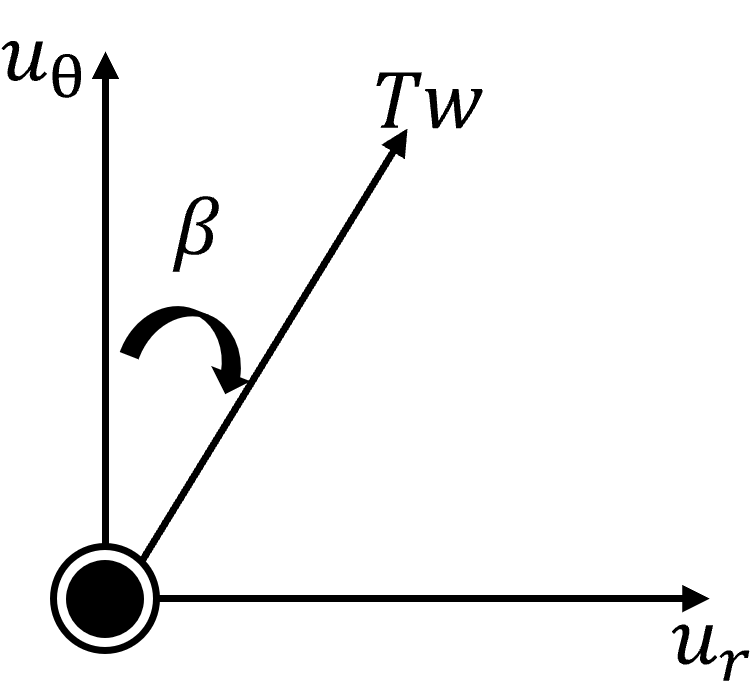
\includegraphics[width=50mm,scale=0.5]{beta.png}
		\caption{Thrust Force at Angle \(\beta\)}
		\label{fig:beta}
	\end{figure}
	\subsection{Position, Velocity and Acceleration of the Spacecraft}
	As seen in Figure \ref{fig:schematic}, the position of the spacecraft represented in reference frame \(A\), is given as 
	\begin{equation} \label{position}
		^A\vec{r}_{P/O} = ru_{r}.
	\end{equation}
	The velocity can then be represented in the inertial frame \(l\) by using equation \ref{golden_rule}, where \(^l\vec{\omega}^A\) is the angular velocity between reference frame \(l\) and \(A\).
	\begin{equation} \label{golden_rule}
		\frac{^ld\vec{r}_{P/O}}{dt} = \frac{^Ad\vec{r}_{P/O}}{dt} +\ ^l\vec{\omega}^A\  \times\  ^A\vec{r}_{P/O} 
	\end{equation}
	Using Equation \ref{golden_rule}, the velocity of the spacecraft in the inertial frame is then formulated as
	\begin{align}
		^l\vec{v_{p}} &= \frac{^ld\vec{r}_{P/O}}{dt} \nonumber\\
		^l\vec{v_{p}} &= \dot{r}u_{r} +\ \dot{\theta}u_{z}\ \times\ ru_{r} \nonumber\\
		^l\vec{v_{p}} &= \dot{r}u_{r} +\ \dot{\theta}ru_{\theta} \label{velocity}
	\end{align}
	The acceleration of the particle can then be formulated as 
	\begin{align}
		^l\vec{a_{p}} &= \frac{^ld\vec{v_{P}}}{dt} \nonumber\\
		^l\vec{a_{p}} &= \frac{^Ad\vec{v_{P}}}{dt} +\ ^l\vec{\omega}^A\  \times\  ^A\vec{v_{P}} \nonumber\\
		^l\vec{a_{p}} &= \ddot{r}u_{r} +\ (\ddot{\theta}r+\dot{\theta}\dot{r})u_{\theta} +\ \dot{\theta}\dot{r}u_{\theta} -\ \dot{\theta}^2ru_{r} \nonumber\\
		^l\vec{a_{p}} &= (\ddot{r} -\ \dot{\theta}^2r)u_{r} +\ (\ddot{\theta}r+2\dot{\theta}\dot{r})u_{\theta}   \label{acceleration}
	\end{align}
	%\[^A\vec{r}_{P/O}\]
	
	%\figurename{Schematic of a particle in a an inertially fixed plane.}
	\subsection{Newton's Second Law for A Particle}
	Newton's second law for a particle is represented by
	\begin{align}
		\sum{F_{P}} = m_{P} * a_{P}. \label{newton}
	\end{align}
	\vspace{2mm}\newline
	Figure \ref{fig:FBD} represents the free body diagram of the particle system. \(F_{G}\), represented by equation \ref{grav_force}, is the gravitational force and acts along the \(u_{r}\) direction. \(F_{T}\), represented by equation \ref{thrust_force}, is the thrust force and acts in the direction \(w\). It can be seen in Figure \ref{fig:beta} that the thrust force can be re-written as 
	\begin{align}
		F_{T} = Tsin(\beta)u_{r} + T\cos(\beta)u_{\theta}, \label{F_T}
	\end{align}
	while the gravitational force can be written as
	\begin{align}
		F_{G} = -m\mu\frac{1}{r^2}u_{r}. \label{F_G}
	\end{align}
	We can now substitute equations \ref{acceleration},  \ref{F_T}, and \ref{F_G} into equation \ref{newton} to obtain
	\begin{align*}
		-m\mu\frac{1}{r^2}u_{r} + Tsin(\beta)u_{r} + T\cos(\beta)u_{\theta} = m[(\ddot{r} -\ \dot{\theta}^2r)u_{r} +\ (\ddot{\theta}r+2\dot{\theta}\dot{r})u_{\theta}]. 
	\end{align*}
	After equating terms, the two equations of motion using Newtons Seconds become:
	\begin{align}
		(u_{r})\qquad      &  \ddot{r}      = \dot{\theta}^2r - \frac{\mu}{r^2} + \frac{Tsin(\beta)}{m} \label{eom1}\\
		(u_{\theta})\qquad &  \ddot{\theta} = -\frac{2\dot{r}\dot{\theta}}{r}   + \frac{T\cos(\beta)}{mr} \label{eom2}
	\end{align}
	\begin{figure}
		%	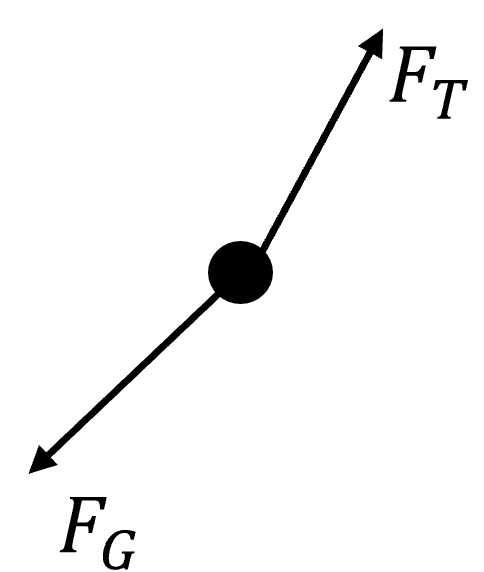
\includegraphics[width=\linewidth]{FBD.png}
		\centering
		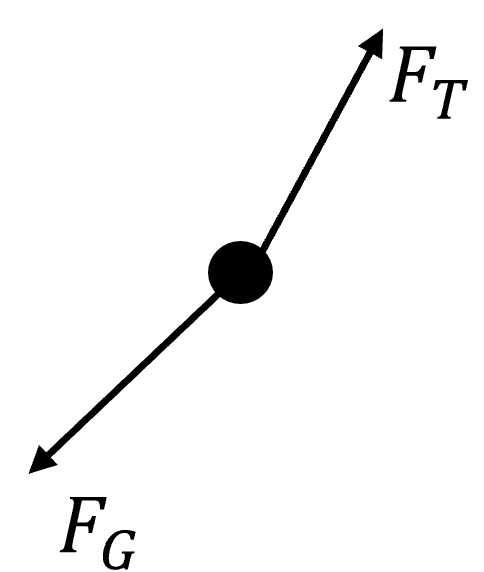
\includegraphics[width=50mm,scale=0.5]{FBD.png}
		\caption{Free Body Diagram}
		\label{fig:FBD}
	\end{figure}

	\subsection{Conversion to First-Order Equations}
	To re-write the two second-order equations into first four first-order equations, the following substitutions can be made:
	\begin{align}
		\dot{r}       &= v_r,     \label{vr} \\
		r\dot{\theta} &= v_\theta,  \nonumber \\
		\dot{\theta}  &= \frac{v_\theta}{r}. \label{vtheta}
	\end{align}
	Then, taking the derivatives of \(r\) and \(\theta\) of equations \ref{vr} and \ref{vtheta}, respectively, we obtain:
	\begin{align}
		\ddot{r}      &= \dot{v}_r,  \label{rddot} \\
		\ddot{\theta} &= \frac{\dot{v}_{\theta}r - v_{\theta}\dot{r}}{r^2}. \label{thetaddot}
	\end{align}
	After substituting equations \ref{vr}, \ref{vtheta}, \ref{rddot}, and \ref{thetaddot} into equations \ref{eom1} and \ref{eom2}, two first-order equations are derived as:
	\begin{align}
		\dot{v}_r     &= \frac{v^2_{\theta}r}{r^2} - \frac{\mu}{r^2} + \frac{T\sin(\beta)}{m},                      \nonumber \\
		\dot{v}_r     &= \frac{v^2_{\theta}}{r} - \frac{\mu}{r^2} + \frac{T\sin(\beta)}{m},                        \label{vrdot}
	\end{align}
	and,
	\begin{align}
		\frac{\dot{v}_{\theta}r - v_{\theta}v_r}{r^2} &= -\frac{2v_{\theta}v_r}{r^2}   + \frac{T\cos(\beta)}{mr},   \nonumber\\
		\dot{v}_{\theta}r - v_{\theta}v_r &= -\frac{2v_{\theta}v_{r}r^2}{r^2}   + \frac{T\cos(\beta)r^2}{mr},       \nonumber\\
		\dot{v}_\theta &= -\frac{2v_{\theta}v_{r}}{r}   + \frac{T\cos(\beta)}{m} + \frac{v_{\theta}v_r}{r},        \nonumber\\
		\dot{v}_\theta &= -\frac{v_{\theta}v_{r}}{r}   + \frac{T\cos(\beta)}{m} \label{vthetadot}.
	\end{align}
	Next, a fifth first-order equation is given as
	\begin{align}
		\dot{m} &= -\frac{T}{v_e}. \label{massflowrate}
	\end{align}
	The five first-order differential equations are listed below:
	\begin{align*}
		\dot{r}       &= v_r,     \\
		\dot{\theta}  &= \frac{v_\theta}{r},  \\ 
	    \dot{v}_r     &= \frac{v^2_{\theta}}{r} - \frac{\mu}{r^2} + \frac{T\sin(\beta)}{m},       \\
		\dot{v}_\theta &= -\frac{v_{\theta}v_{r}}{r}   + \frac{T\cos(\beta)}{m}, \\
		\dot{m} &= -\frac{T}{v_e}.
	\end{align*}

	\section{Formulation of Optimal Control Problem}
	There are two objectives for the optimal control problem. The first objective is to minimize the time to transfer from an initial circular orbit to a final circular orbit. The second objective is to maximize the terminal mass when transferring from an initial circular orbit to a final circular orbit. Below is an overview of the problem:
\begin{align*}
	\mathrm{Objective \ 1}:& \quad \min\ t_f \\
	\mathrm{Objective \ 2}:& \quad \max\ m(t_f) \\
	\mathrm{State}:&     \quad r(t), \theta(t), v_r(t), v_\theta(t), m(t) \\
	\mathrm{Control}:&   \quad \beta(t), T(t)
\end{align*}

	\section{Numerical Solution of Optimal Control Problem}
	The optimal control problem was solved using multiple interval Legendre-Gauss-Radau collocation. For simplicity, Adigator was used for automatic differentiation and IPOPT was used for the nonlinear optimization. For this study, four different cases were investigated. The four different discretizations of Legendre-Gauss-Radau collocation are:
	\begin{enumerate}
		\item Minimize \(t_f\) with with unconstrained control parameterized by polynomial degrees N = (3,4) with intervals of K = (2,4,8,16,32)
		\item Minimize \(m(t_f)\) with with unconstrained control parameterized by polynomial degrees N = (3,4) with intervals of K = (2,4,8,16,32)
		\item Minimize \(t_f\) with with constrained control parameterized by polynomial degrees N = (3,4) with intervals of K = (2,4,8,16,32)
		\item Minimize \(m(t_f)\) with with constrained control parameterized by polynomial degrees N = (3,4) with intervals of K = (2,4,8,16,32)
	\end{enumerate}
%         0  solved
%         1  solved to acceptable level
%         2  infeasible problem detected
%         3  search direction becomes too small
%         4  diverging iterates
%         5  user requested stop
%     
%        -1  maximum number of iterations exceeded
%        -2  restoration phase failed
%        -3  error in step computation
    \subsection{Minimize Terminal Time with Unconstrained Control}
\begin{figure}
	\centering
	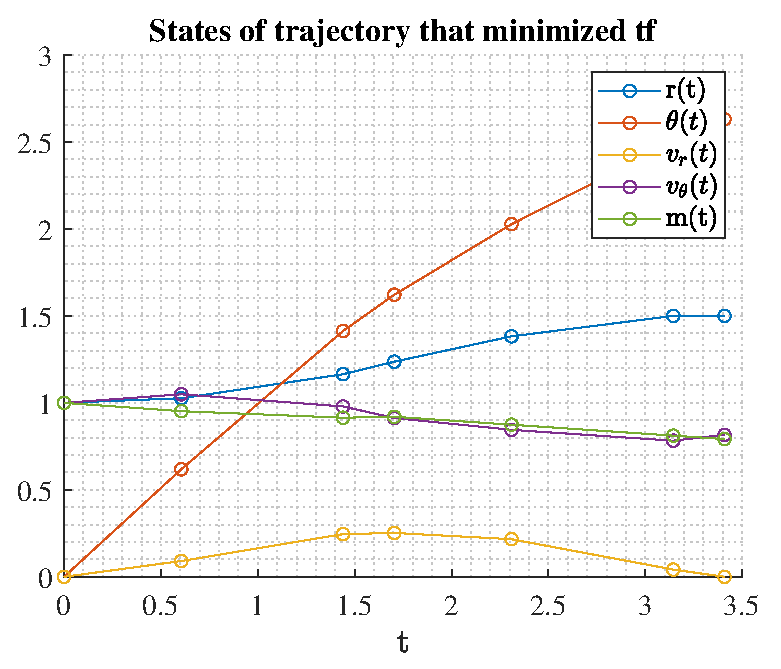
\includegraphics[scale=0.75]{states_N3_K2_C2_tf.eps}
	\caption{States for trajectory that minimized terminal time (\(N:3\ , K:2\))}
	\label{fig:states_N3_K2_C2_tf}
\end{figure}
\begin{figure}
	\centering
	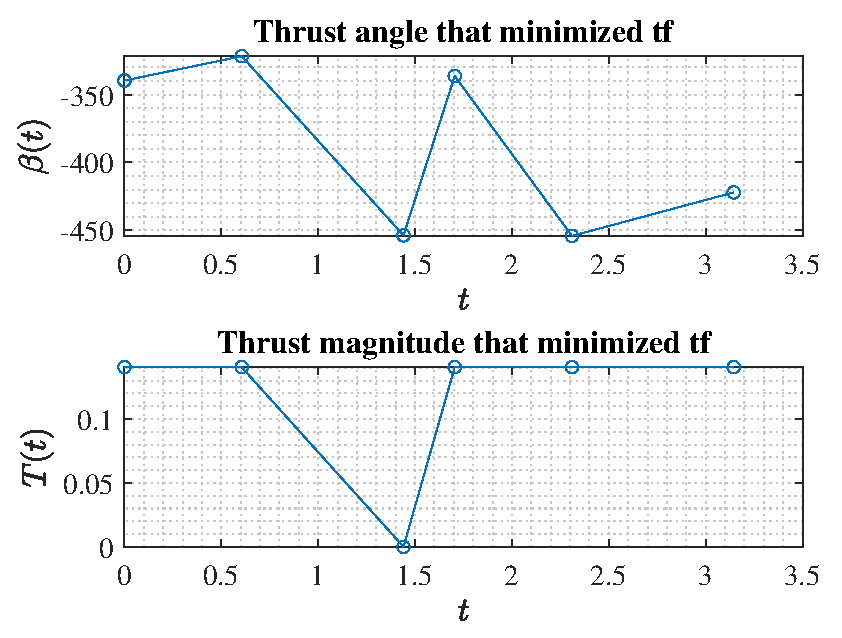
\includegraphics[scale=0.75]{control_N3_K2_C2_tf.eps}
	\caption{Control that minimized terminal time (\(N:3\ , K:2\))}
	\label{fig:control_N3_K2_C2_tf}
\end{figure}
\begin{figure}
	\centering
	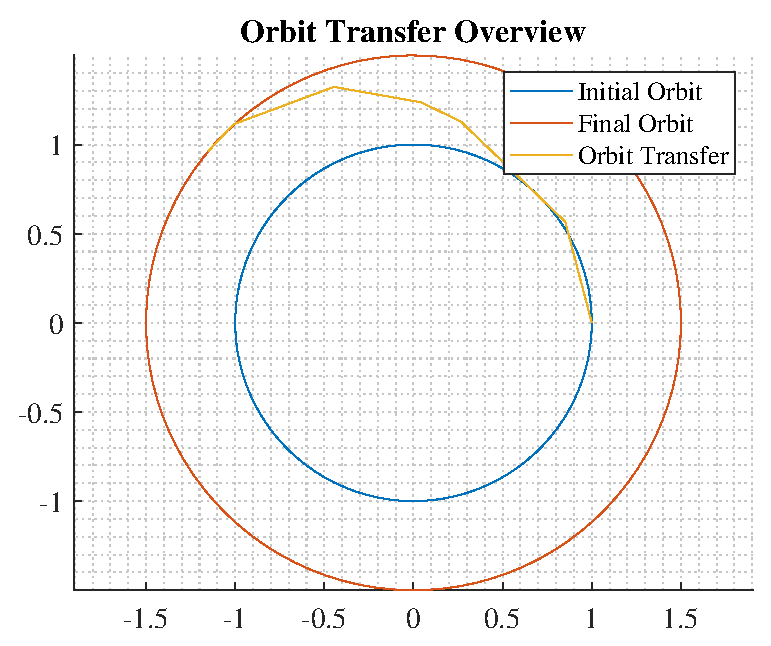
\includegraphics[scale=0.75]{orbit_N3_K2_C2_tf.eps}
	\caption{Trajectory from initial to final orbit (\(N:3\ , K:2\))}
	\label{fig:orbit_N3_K2_C2_tf}
\end{figure}
\begin{figure}
	\centering
	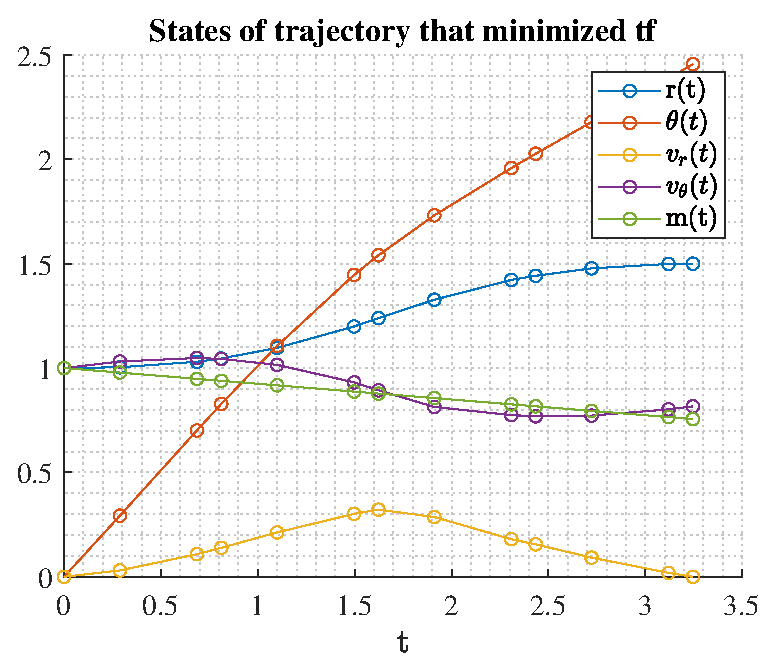
\includegraphics[scale=0.75]{states_N3_K4_C2_tf.eps}
	\caption{States for trajectory that minimized terminal time (\(N:3\ , K:4\))}
	\label{fig:states_N3_K4_C2_tf}
\end{figure}
\begin{figure}
	\centering
	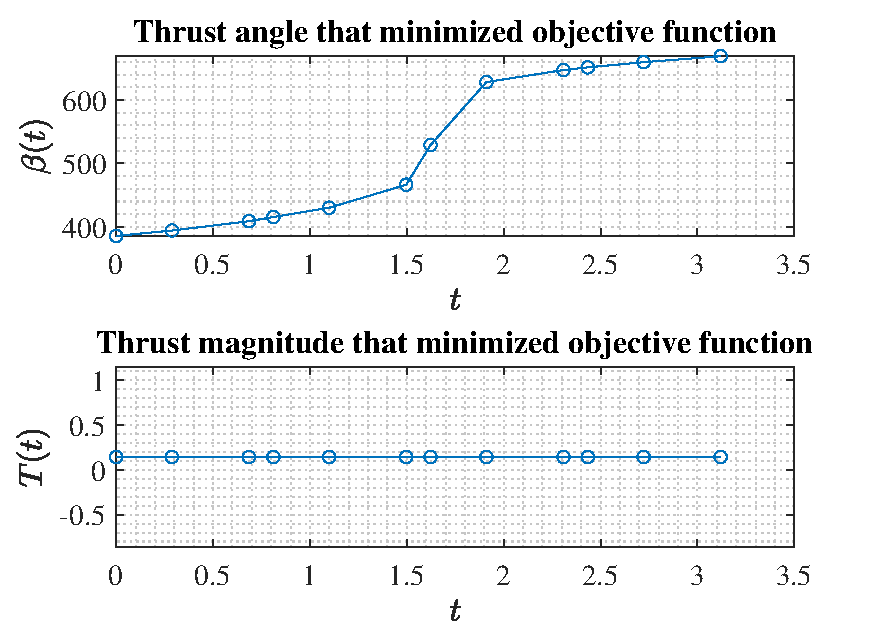
\includegraphics[scale=0.75]{control_N3_K4_C2_tf.eps}
	\caption{Control that minimized terminal time (\(N:3\ , K:4\))}
	\label{fig:control_N3_K4_C2_tf}
\end{figure}
\begin{figure}
	\centering
	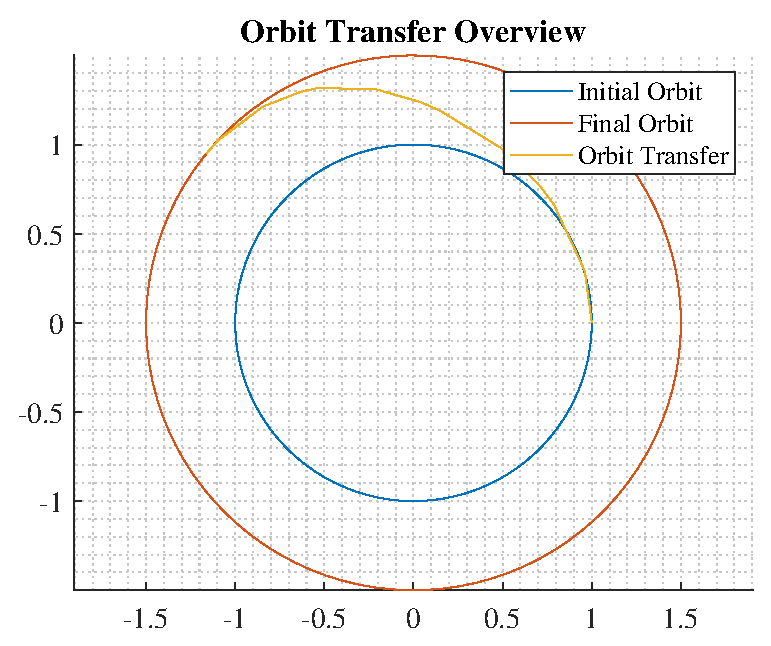
\includegraphics[scale=0.75]{orbit_N3_K4_C2_tf.eps}
	\caption{Trajectory from initial to final orbit (\(N:3\ , K:4\))}
	\label{fig:orbit_N3_K4_C2_tf}
\end{figure}
\begin{figure}
	\centering
	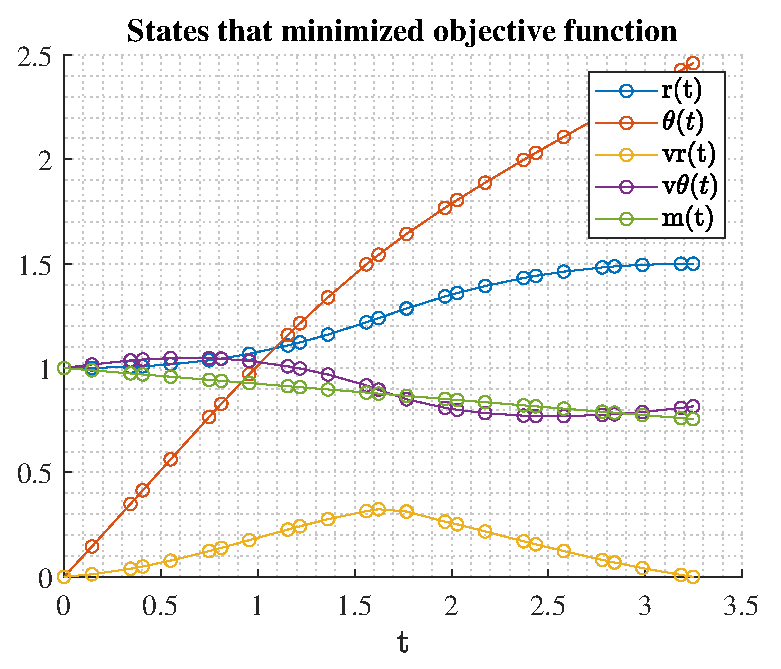
\includegraphics[scale=0.75]{states_N3_K8_C2_tf.eps}
	\caption{States for trajectory that minimized terminal time (\(N:3\ , K:8\))}
	\label{fig:states_N3_K8_C2_tf}
\end{figure}
\begin{figure}
	\centering
	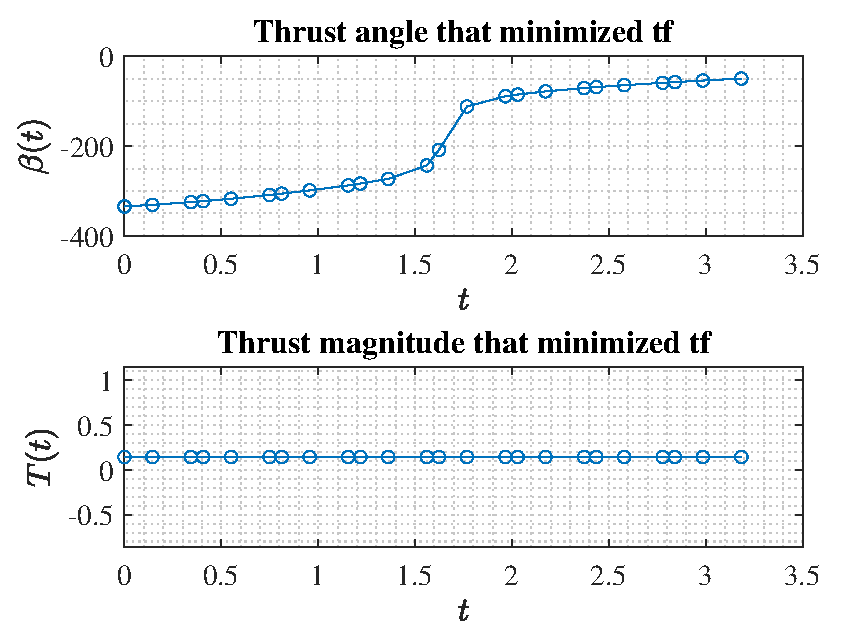
\includegraphics[scale=0.75]{control_N3_K8_C2_tf.eps}
	\caption{Control that minimized terminal time (\(N:3\ , K:8\))}
	\label{fig:control_N3_K8_C2_tf}
\end{figure}
\begin{figure}
	\centering
	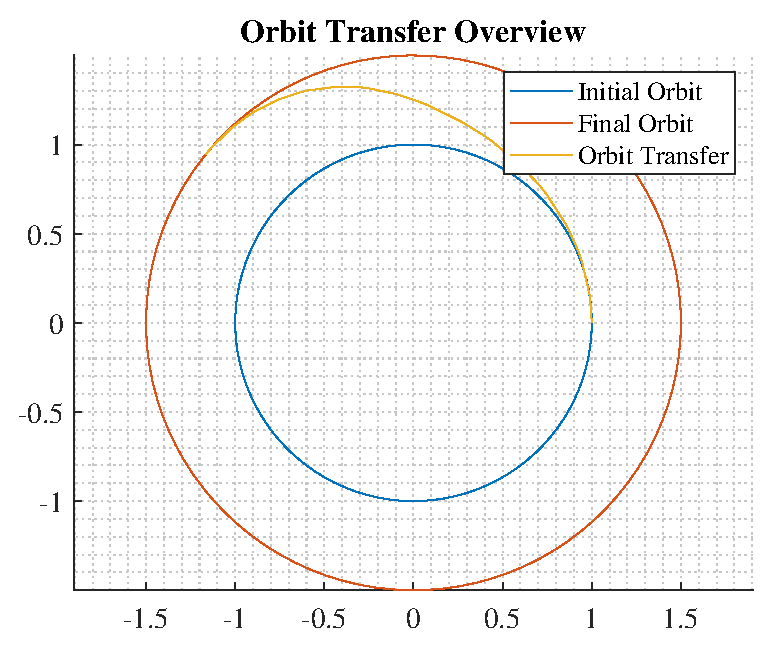
\includegraphics[scale=0.75]{orbit_N3_K8_C2_tf.eps}
	\caption{Trajectory from initial to final orbit (\(N:3\ , K:8\))}
	\label{fig:orbit_N3_K8_C2_tf}
\end{figure}
\begin{figure}
	\centering
	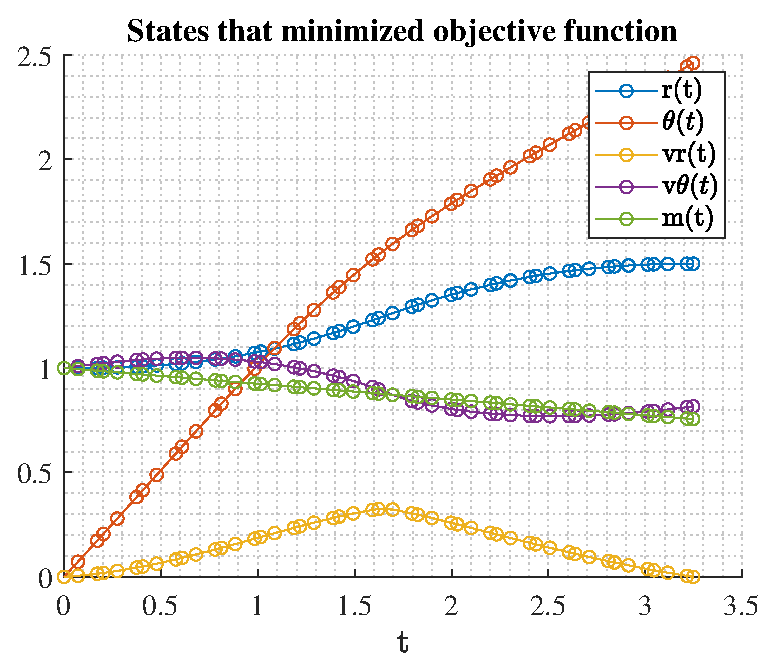
\includegraphics[scale=0.75]{states_N3_K16_C2_tf.eps}
	\caption{States for trajectory that minimized terminal time (\(N:3\ , K:16\))}
	\label{fig:states_N3_K16_C2_tf}
\end{figure}
\begin{figure}
	\centering
	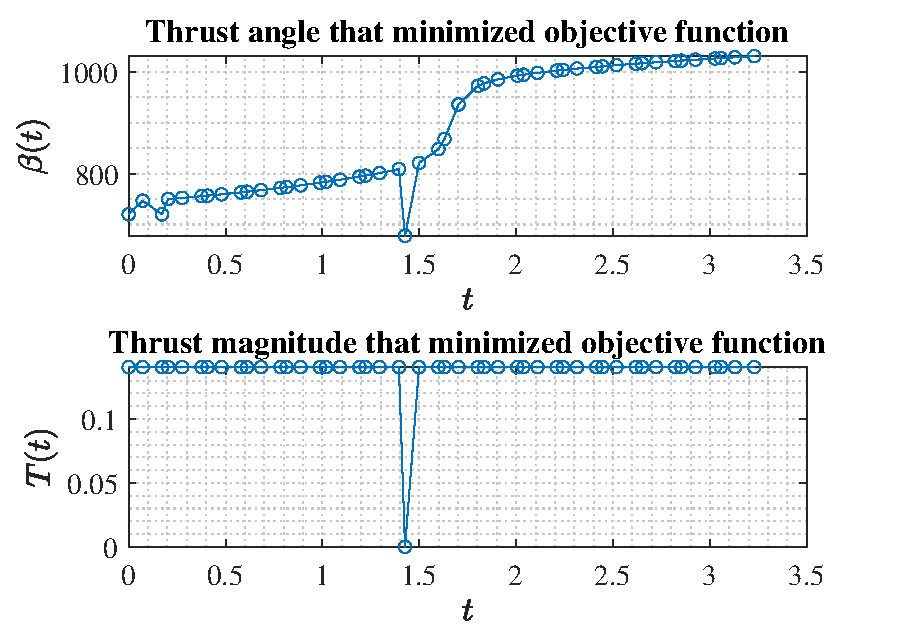
\includegraphics[scale=0.75]{control_N3_K16_C2_tf.eps}
	\caption{Control that minimized terminal time (\(N:3\ , K:16\))}
	\label{fig:control_N3_K16_C2_tf}
\end{figure}
\begin{figure}
	\centering
	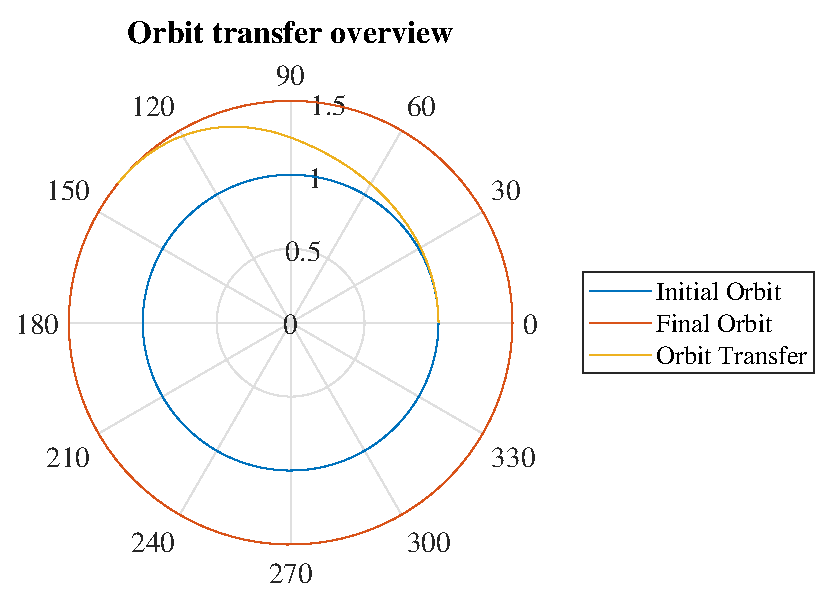
\includegraphics[scale=0.75]{orbit_N3_K16_C2_tf.eps}
	\caption{Trajectory from initial to final orbit (\(N:3\ , K:16\))}
	\label{fig:orbit_N3_K16_C2_tf}
\end{figure}
\begin{figure}
	\centering
	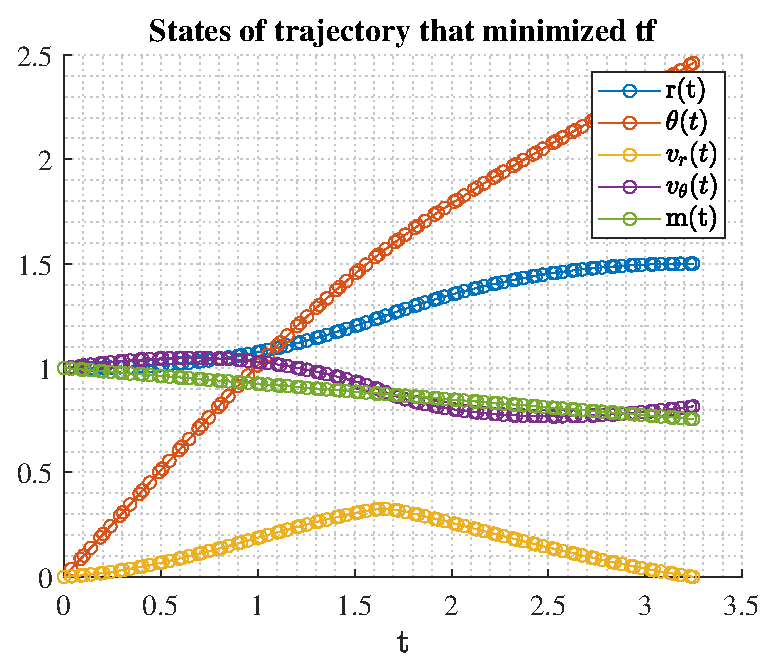
\includegraphics[scale=0.75]{states_N3_K32_C2_tf.eps}
	\caption{States for trajectory that minimized terminal time (\(N:3\ , K:32\))}
	\label{fig:states_N3_K32_C2_tf}
\end{figure}
\begin{figure}
	\centering
	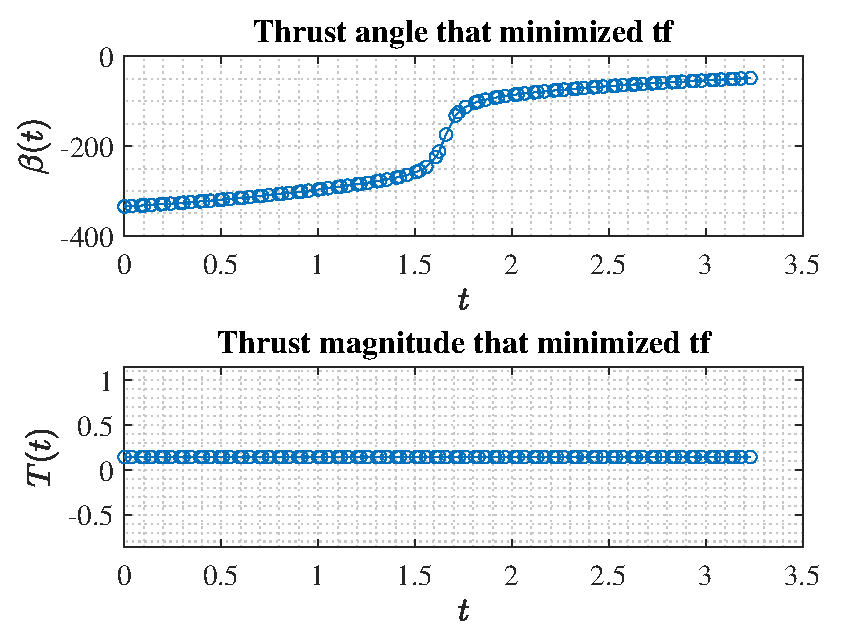
\includegraphics[scale=0.75]{control_N3_K32_C2_tf.eps}
	\caption{Control that minimized terminal time (\(N:3\ , K:32\))}
	\label{fig:control_N3_K32_C2_tf}
\end{figure}
\begin{figure}
	\centering
	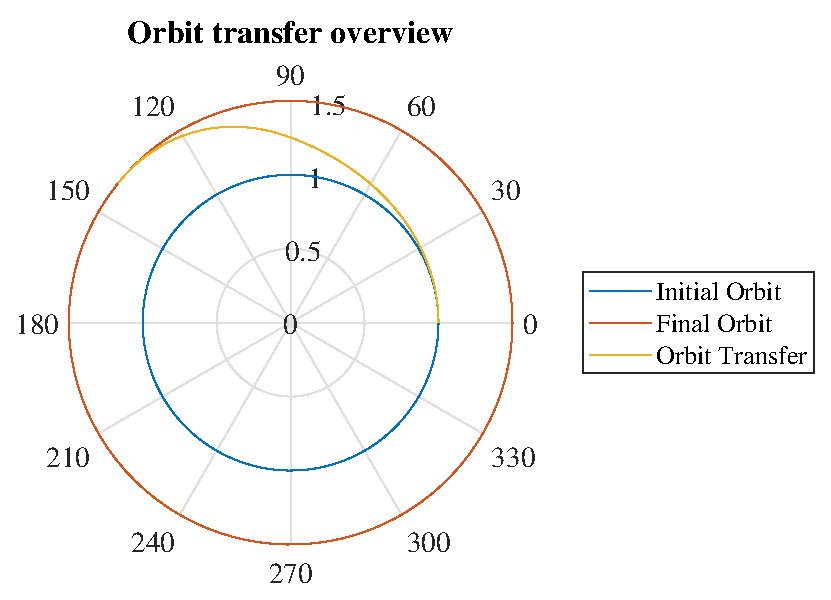
\includegraphics[scale=0.75]{orbit_N3_K32_C2_tf.eps}
	\caption{Trajectory from initial to final orbit (\(N:3\ , K:32\))}
	\label{fig:orbit_N3_K32_C2_tf}
\end{figure}
\begin{figure}
	\centering
	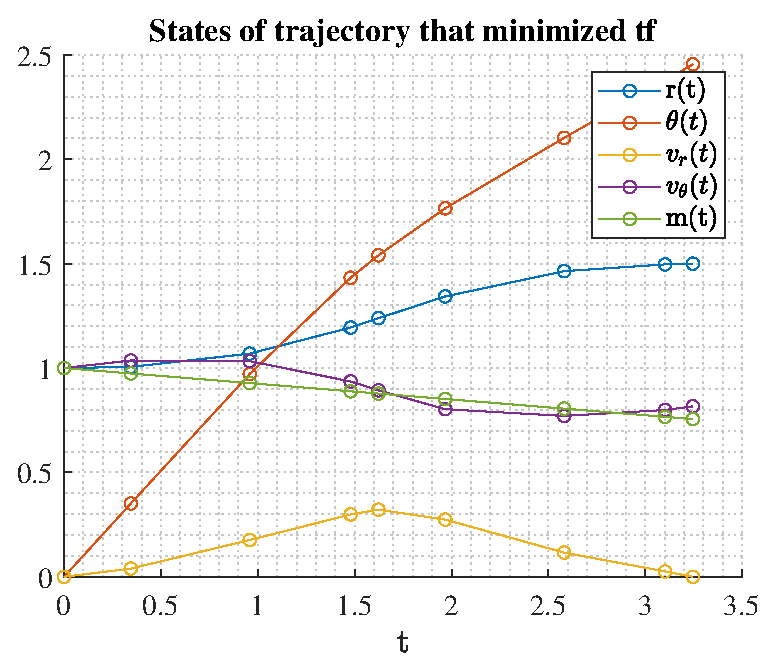
\includegraphics[scale=0.75]{states_N4_K2_C2_tf.eps}
	\caption{States for trajectory that minimized terminal time (\(N:4\ , K:2\))}
	\label{fig:states_N4_K2_C2_tf}
\end{figure}
\begin{figure}
	\centering
	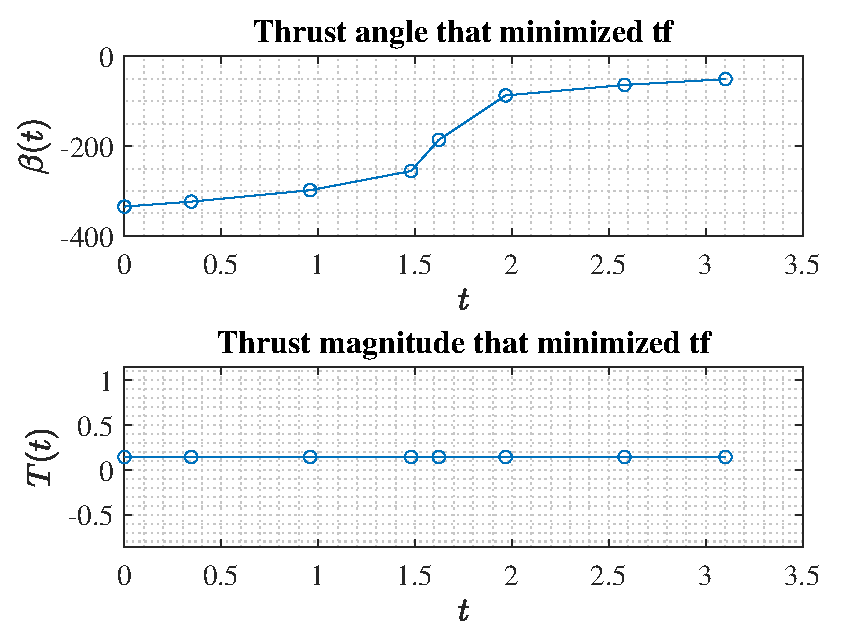
\includegraphics[scale=0.75]{control_N4_K2_C2_tf.eps}
	\caption{Control that minimized terminal time (\(N:4\ , K:2\))}
	\label{fig:control_N4_K2_C2_tf}
\end{figure}
\begin{figure}
	\centering
	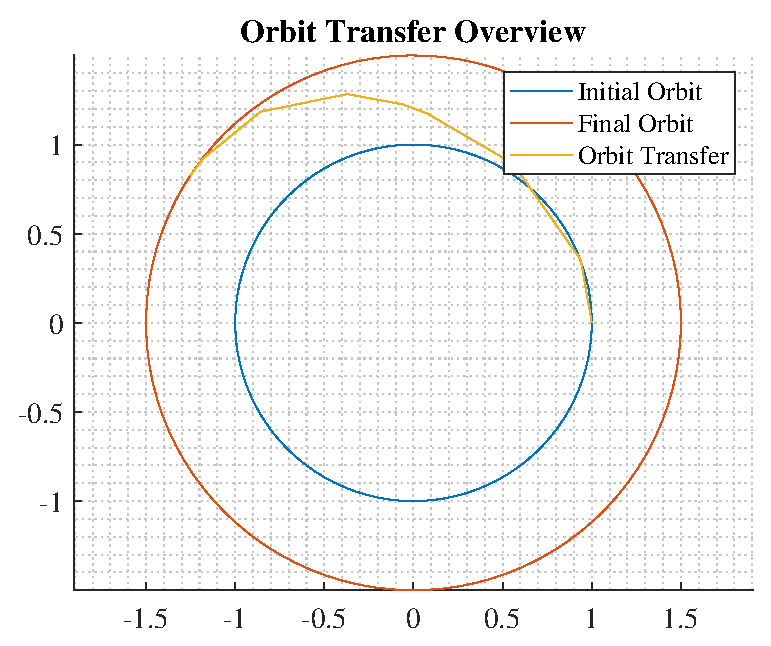
\includegraphics[scale=0.75]{orbit_N4_K2_C2_tf.eps}
	\caption{Trajectory from initial to final orbit (\(N:4\ , K:2\))}
	\label{fig:orbit_N4_K2_C2_tf}
\end{figure}
\begin{figure}
	\centering
	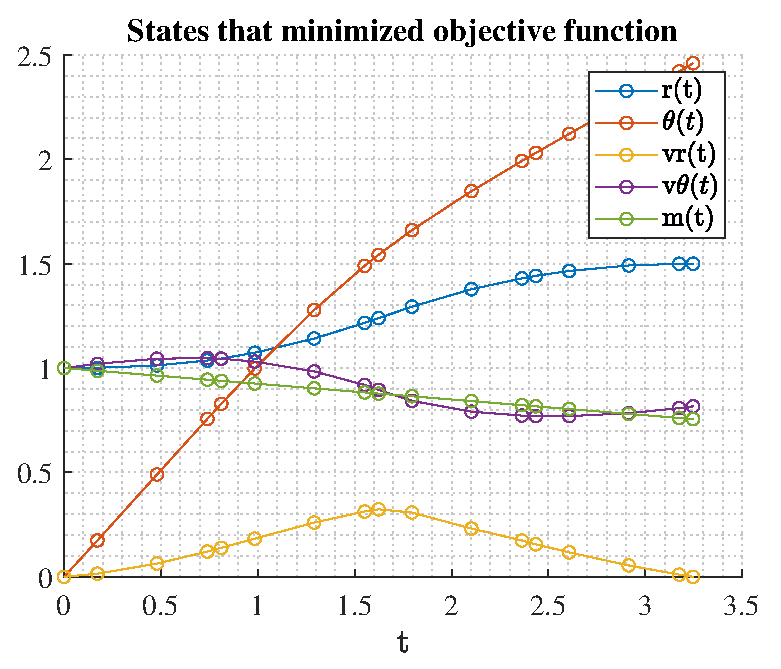
\includegraphics[scale=0.75]{states_N4_K4_C2_tf.eps}
	\caption{States for trajectory that minimized terminal time (\(N:4\ , K:4\))}
	\label{fig:states_N4_K4_C2_tf}
\end{figure}
\begin{figure}
	\centering
	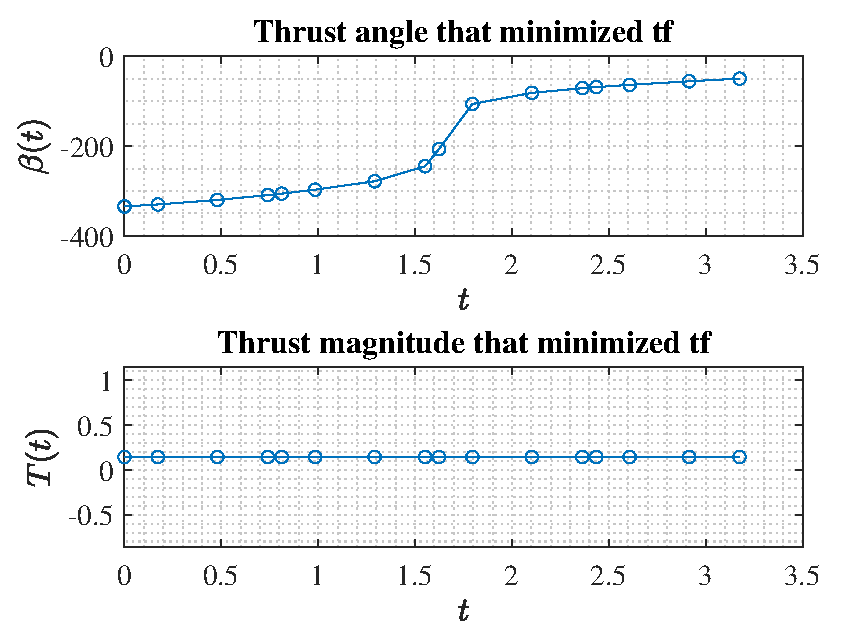
\includegraphics[scale=0.75]{control_N4_K4_C2_tf.eps}
	\caption{Control that minimized terminal time (\(N:4\ , K:4\))}
	\label{fig:control_N4_K4_C2_tf}
\end{figure}
\begin{figure}
	\centering
	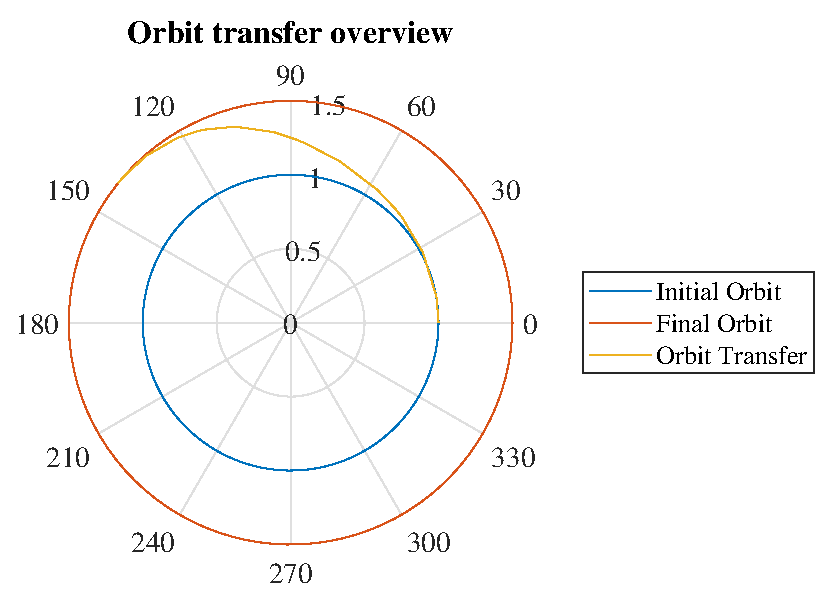
\includegraphics[scale=0.75]{orbit_N4_K4_C2_tf.eps}
	\caption{Trajectory from initial to final orbit (\(N:4\ , K:4\))}
	\label{fig:orbit_N4_K4_C2_tf}
\end{figure}
\begin{figure}
	\centering
	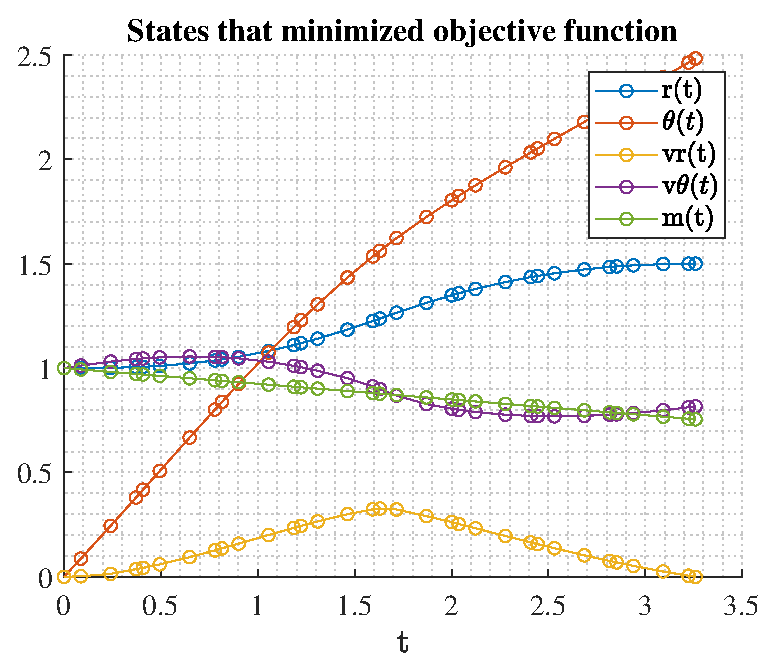
\includegraphics[scale=0.75]{states_N4_K8_C2_tf.eps}
	\caption{States for trajectory that minimized terminal time (\(N:4\ , K:8\))}
	\label{fig:states_N4_K8_C2_tf}
\end{figure}
\begin{figure}
	\centering
	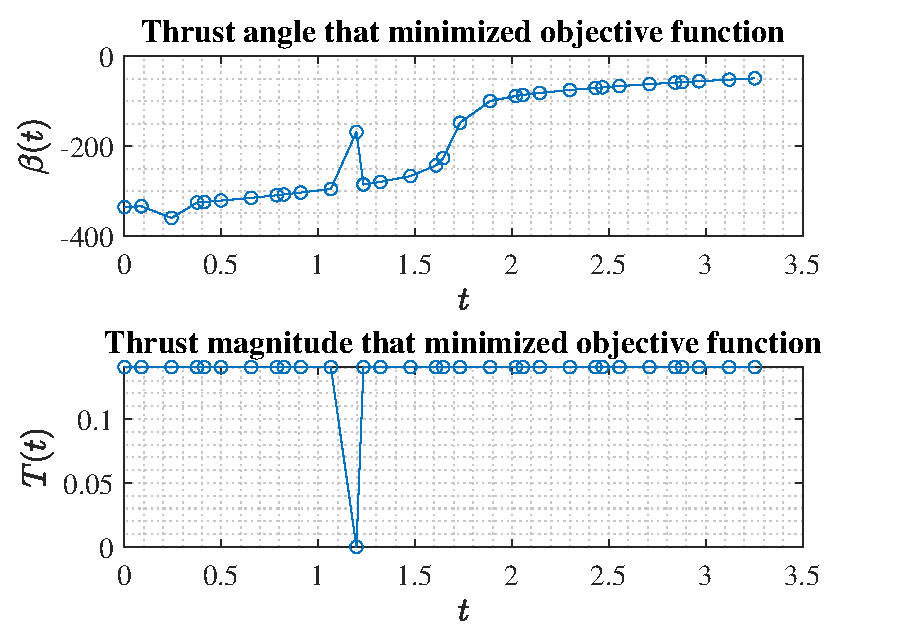
\includegraphics[scale=0.75]{control_N4_K8_C2_tf.eps}
	\caption{Control that minimized terminal time (\(N:4\ , K:8\))}
	\label{fig:control_N4_K8_C2_tf}
\end{figure}
\begin{figure}
	\centering
	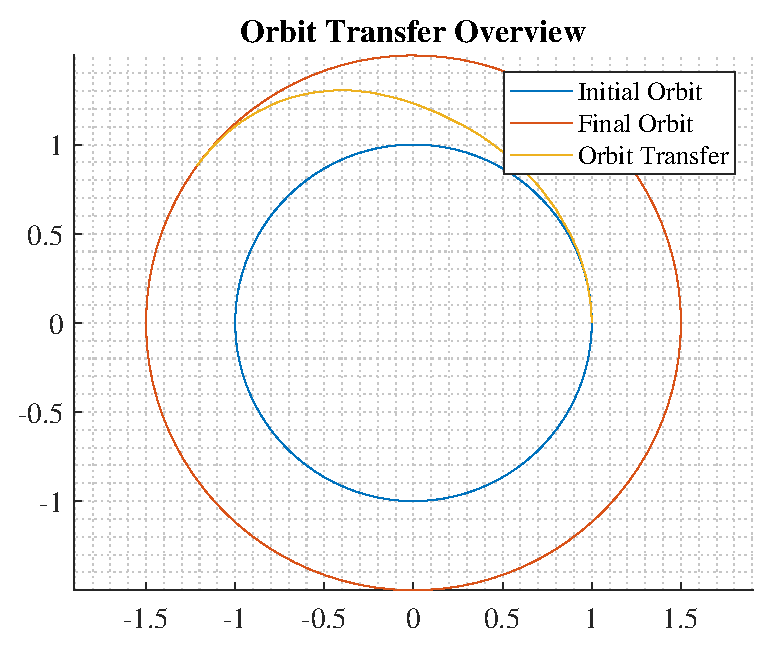
\includegraphics[scale=0.75]{orbit_N4_K8_C2_tf.eps}
	\caption{Trajectory from initial to final orbit (\(N:4\ , K:8\))}
	\label{fig:orbit_N4_K8_C2_tf}
\end{figure}
\begin{figure}
	\centering
	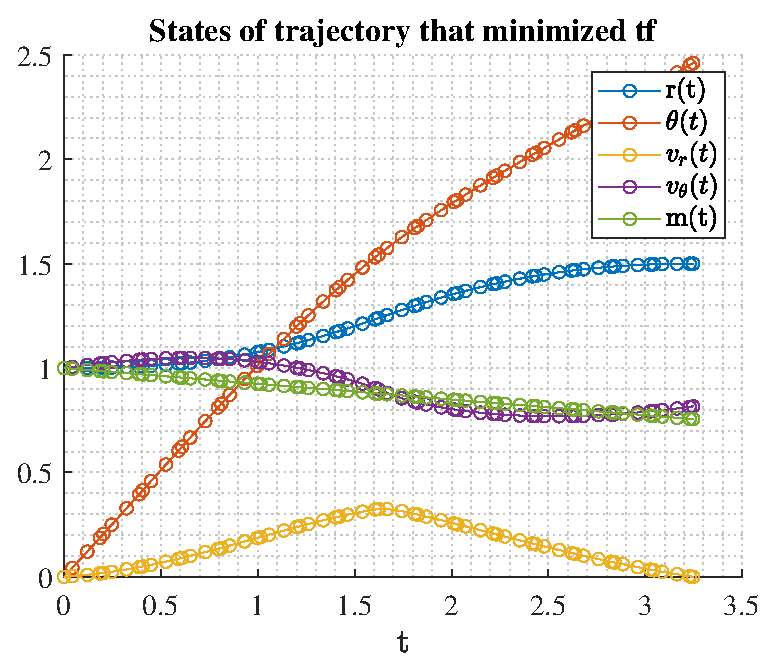
\includegraphics[scale=0.75]{states_N4_K16_C2_tf.eps}
	\caption{States for trajectory that minimized terminal time (\(N:4\ , K:16\))}
	\label{fig:states_N4_K16_C2_tf}
\end{figure}
\begin{figure}
	\centering
	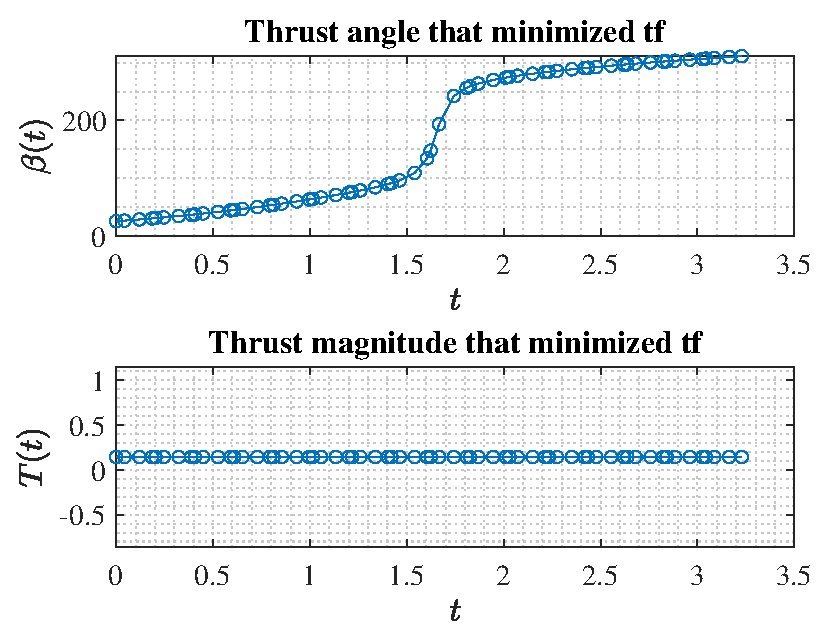
\includegraphics[scale=0.75]{control_N4_K16_C2_tf.eps}
	\caption{Control that minimized terminal time (\(N:4\ , K:16\))}
	\label{fig:control_N4_K16_C2_tf}
\end{figure}
\begin{figure}
	\centering
	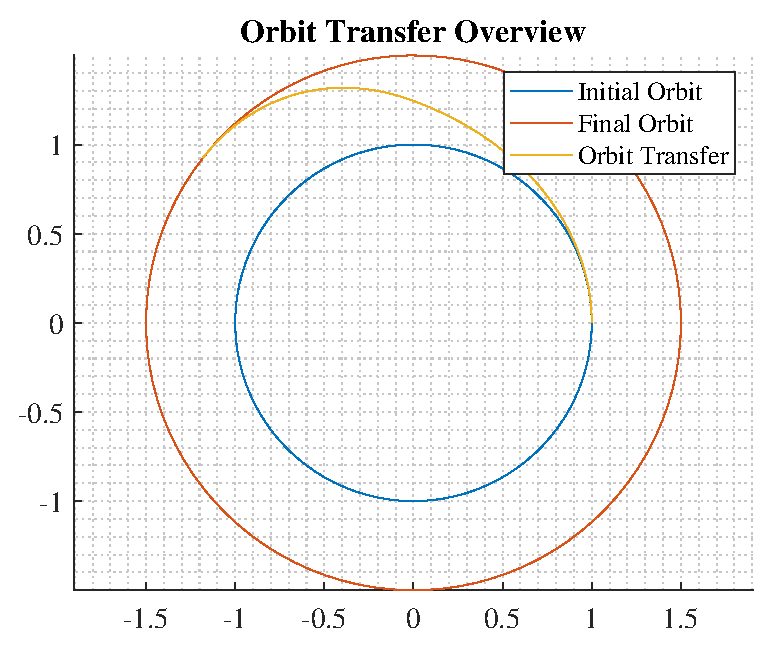
\includegraphics[scale=0.75]{orbit_N4_K16_C2_tf.eps}
	\caption{Trajectory from initial to final orbit (\(N:4\ , K:16\))}
	\label{fig:orbit_N4_K16_C2_tf}
\end{figure}
\begin{figure}
	\centering
	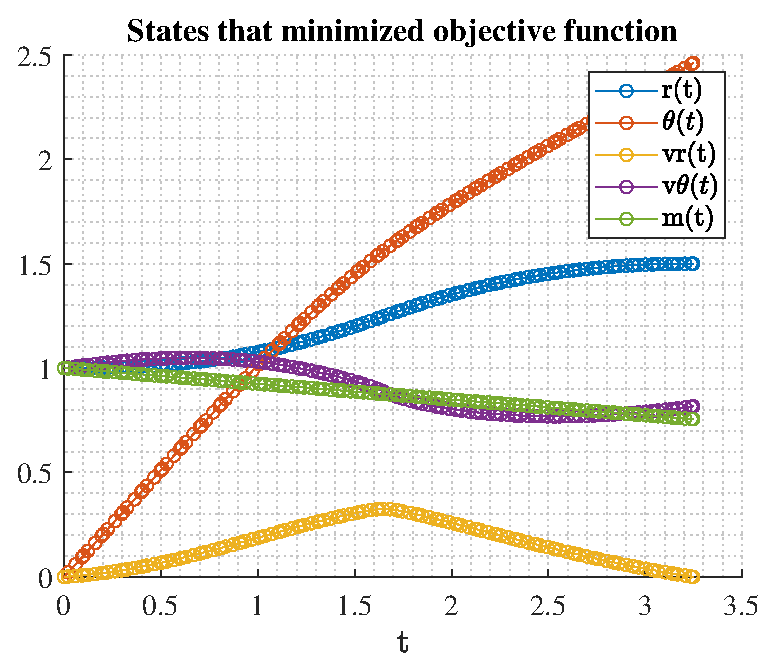
\includegraphics[scale=0.75]{states_N4_K32_C2_tf.eps}
	\caption{States for trajectory that minimized terminal time (\(N:4\ , K:32\))}
	\label{fig:states_N4_K32_C2_tf}
\end{figure}
\begin{figure}
	\centering
	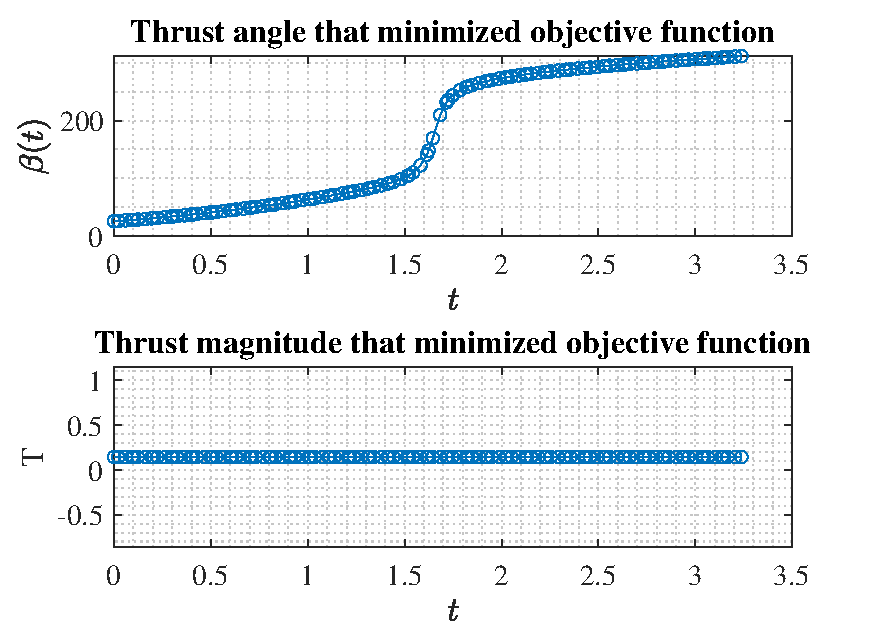
\includegraphics[scale=0.75]{control_N4_K32_C2_tf.eps}
	\caption{Control that minimized terminal time (\(N:4\ , K:32\))}
	\label{fig:control_N4_K32_C2_tf}
\end{figure}
\begin{figure}
	\centering
	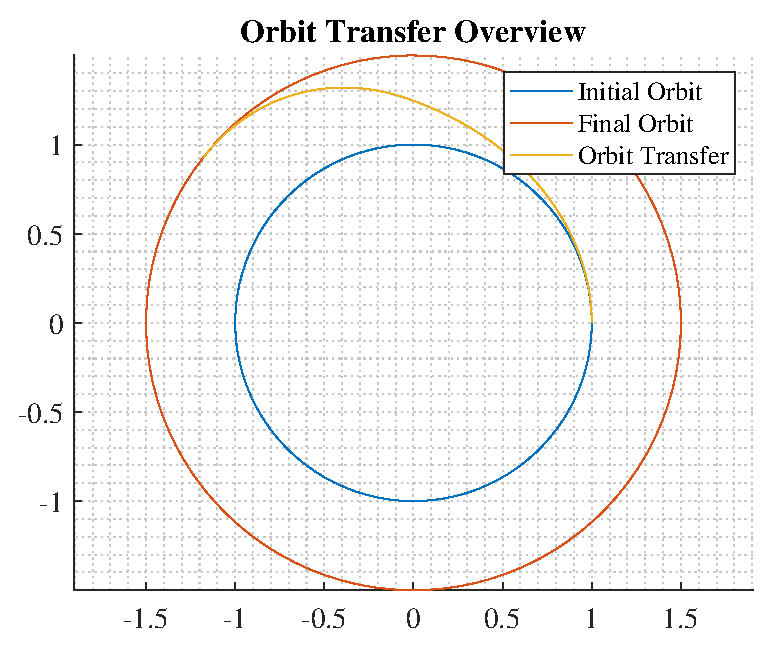
\includegraphics[scale=0.75]{orbit_N4_K32_C2_tf.eps}
	\caption{Trajectory from initial to final orbit (\(N:4\ , K:32\))}
	\label{fig:orbit_N4_K32_C2_tf}
\end{figure}
\begin{table}
	\begin{tabular}{lllllll}
		Degree & Intervals & Iterations & CPU Time & tf & mf & Solved\ Status \\ 
		\hline 
		3 & 2 & 35 & 0.185 & 3.2444 & 0.75569 & 0 \\ 
		3 & 4 & 66 & 0.427 & 3.2457 & 0.75559 & 0 \\ 
		3 & 8 & 155 & 0.623 & 3.3381 & 0.74864 & 0 \\ 
		3 & 16 & 110 & 0.499 & 3.2605 & 0.75619 & 0 \\ 
		3 & 32 & 187 & 0.893 & 3.2479 & 0.75543 & 0 \\ 
		4 & 2 & 80 & 0.337 & 3.31 & 0.75075 & 0 \\ 
		4 & 4 & 153 & 0.588 & 3.2466 & 0.75552 & 0 \\ 
		4 & 8 & 126 & 0.54 & 3.2896 & 0.75912 & 0 \\ 
		4 & 16 & 144 & 0.659 & 3.2567 & 0.75572 & 0 \\ 
		4 & 32 & 174 & 0.952 & 3.2546 & 0.75492 & 1 \\ 
		\hline 
	\end{tabular}
	\caption{Results for minimizing \(t_f\) with unconstrained control}
	\label{table:1}
\end{table}
\FloatBarrier
	\subsection{Maximize Terminal Mass with Unconstrained Control}
\begin{figure}
	\centering
	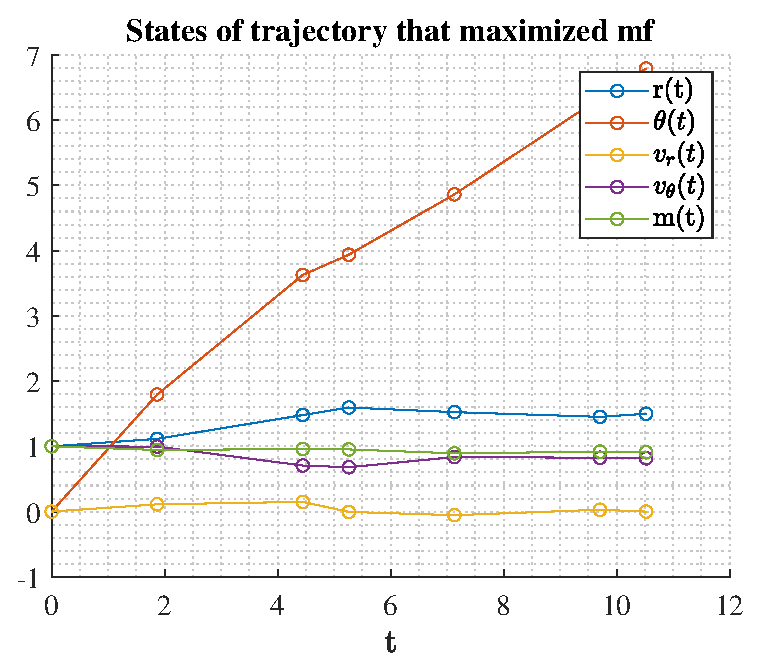
\includegraphics[scale=0.75]{states_N3_K2_C2_mf.eps}
	\caption{States for trajectory that maximized terminal mass (\(N:3\ , K:2\))}
	\label{fig:states_N3_K2_C2_mf}
\end{figure}
\begin{figure}
	\centering
	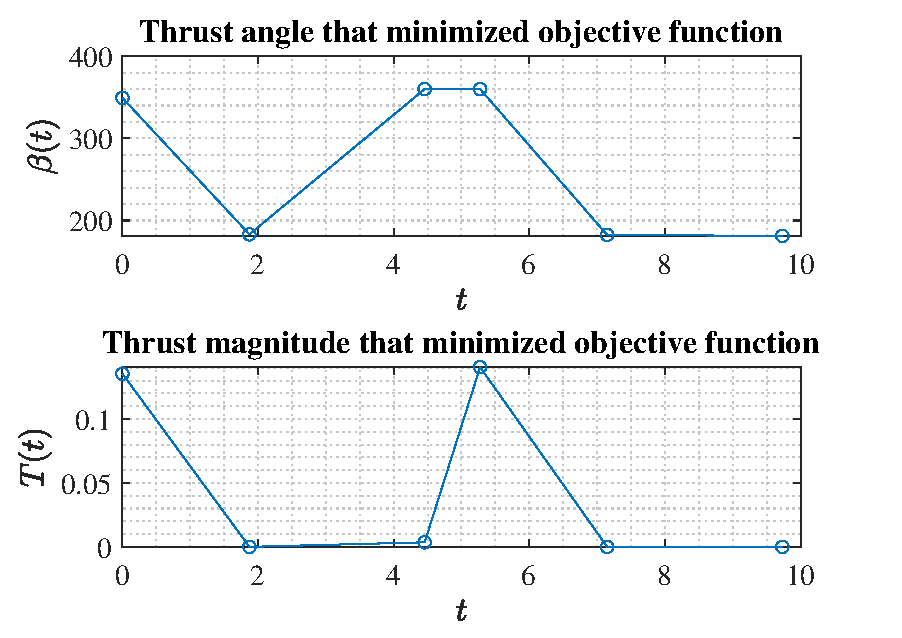
\includegraphics[scale=0.75]{control_N3_K2_C2_mf.eps}
	\caption{Control that maximized terminal mass (\(N:3\ , K:2\))}
	\label{fig:control_N3_K2_C2_mf}
\end{figure}
\begin{figure}
	\centering
	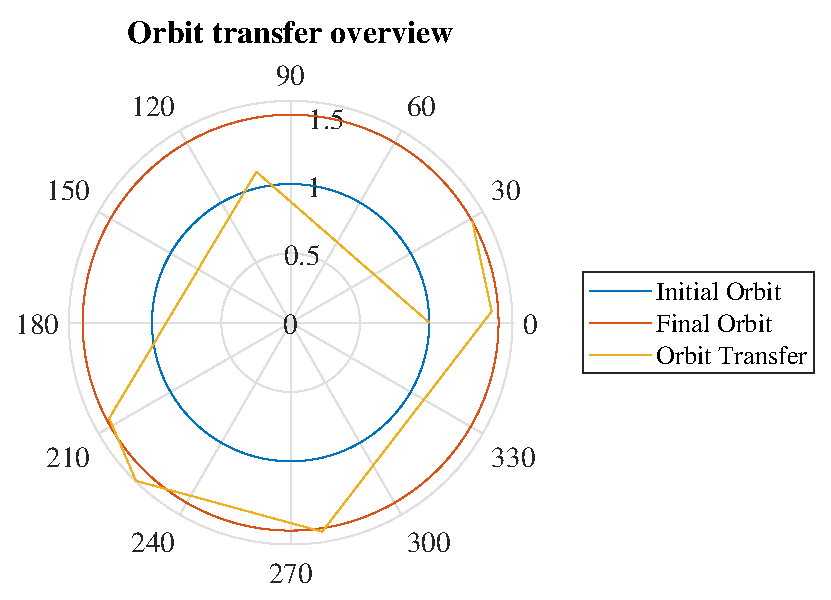
\includegraphics[scale=0.75]{orbit_N3_K2_C2_mf.eps}
	\caption{Trajectory from initial to final orbit (\(N:3\ , K:2\))}
	\label{fig:orbit_N3_K2_C2_mf}
\end{figure}
\begin{figure}
	\centering
	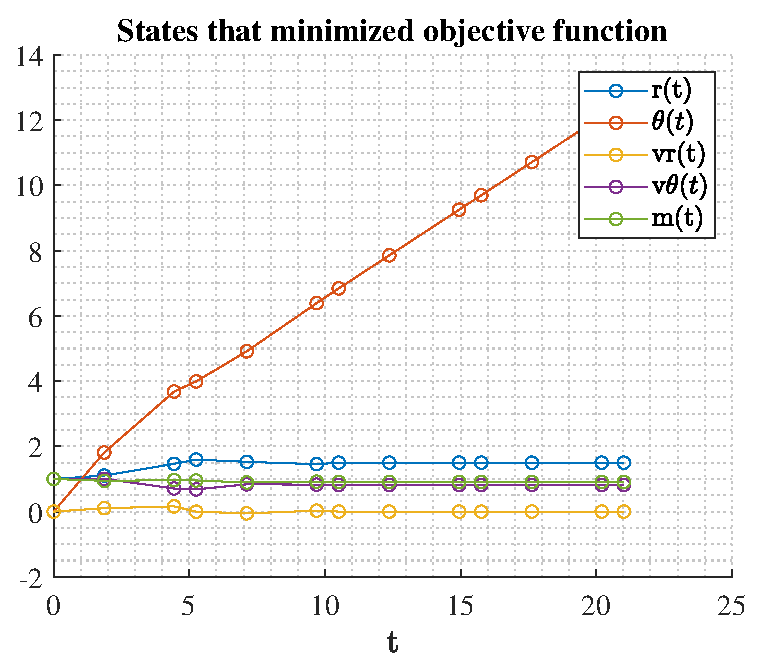
\includegraphics[scale=0.75]{states_N3_K4_C2_mf.eps}
	\caption{States for trajectory that maximized terminal mass (\(N:3\ , K:4\))}
	\label{fig:states_N3_K4_C2_mf}
\end{figure}
\begin{figure}
	\centering
	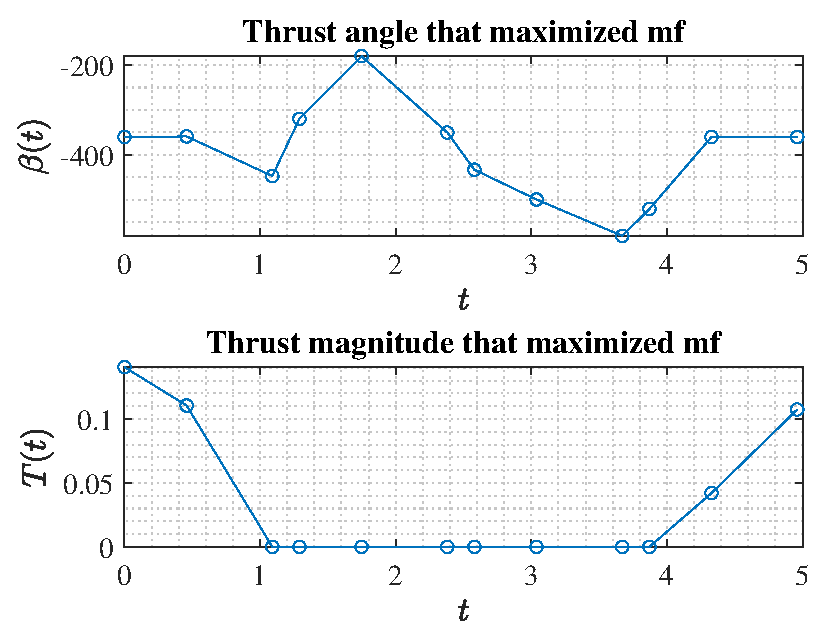
\includegraphics[scale=0.75]{control_N3_K4_C2_mf.eps}
	\caption{Control that maximized terminal mass (\(N:3\ , K:4\))}
	\label{fig:control_N3_K4_C2_mf}
\end{figure}
\begin{figure}
	\centering
	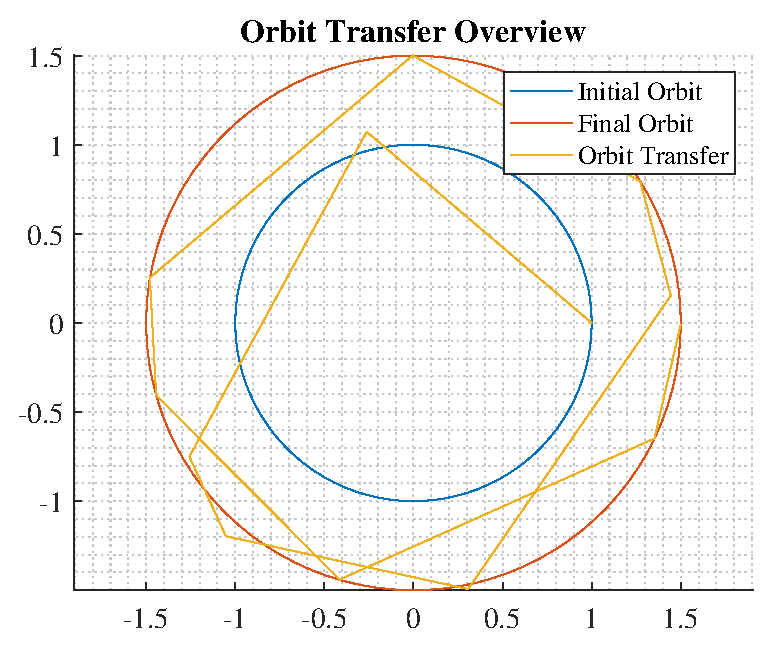
\includegraphics[scale=0.75]{orbit_N3_K4_C2_mf.eps}
	\caption{Trajectory from initial to final orbit (\(N:3\ , K:4\))}
	\label{fig:orbit_N3_K4_C2_mf}
\end{figure}
\begin{figure}
	\centering
	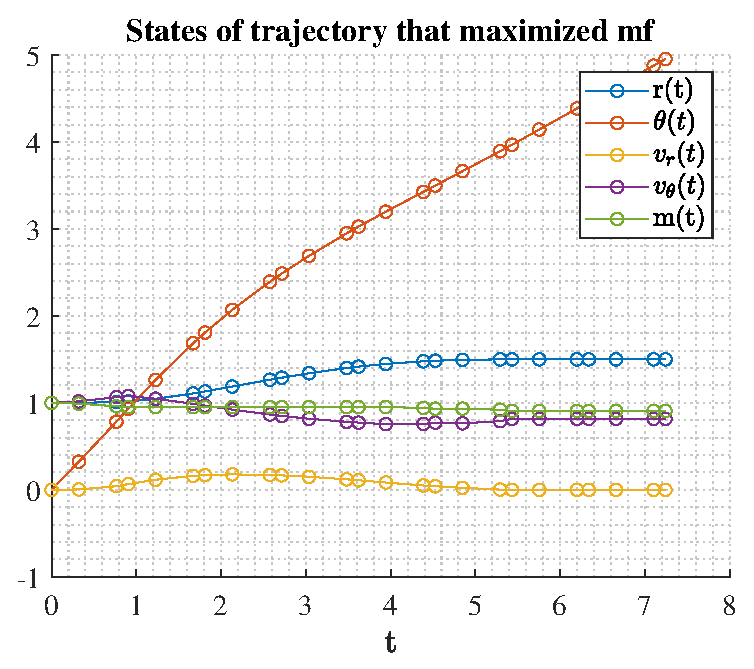
\includegraphics[scale=0.75]{states_N3_K8_C2_mf.eps}
	\caption{States for trajectory that maximized terminal mass (\(N:3\ , K:8\))}
	\label{fig:states_N3_K8_C2_mf}
\end{figure}
\begin{figure}
	\centering
	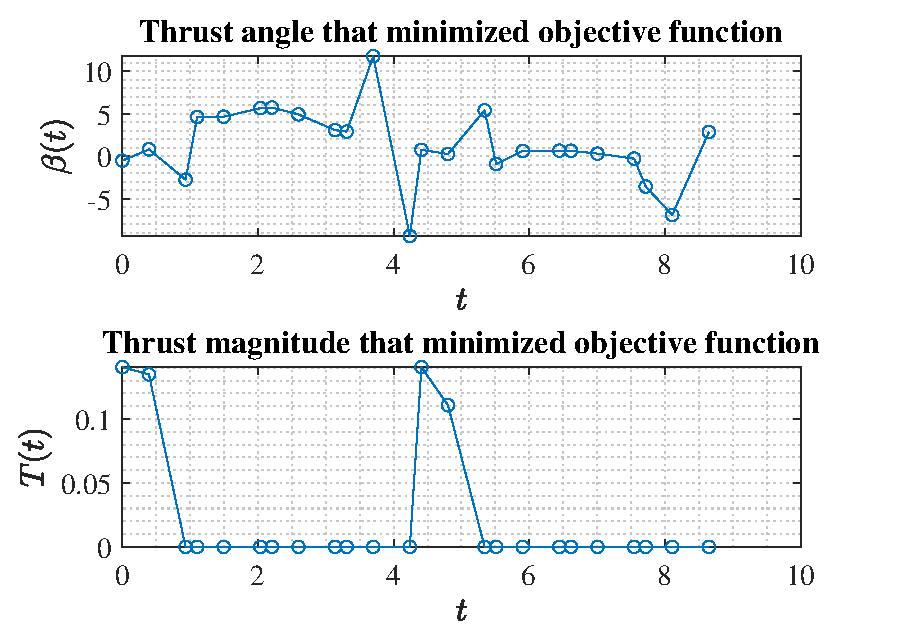
\includegraphics[scale=0.75]{control_N3_K8_C2_mf.eps}
	\caption{Control that maximized terminal mass (\(N:3\ , K:8\))}
	\label{fig:control_N3_K8_C2_mf}
\end{figure}
\begin{figure}
	\centering
	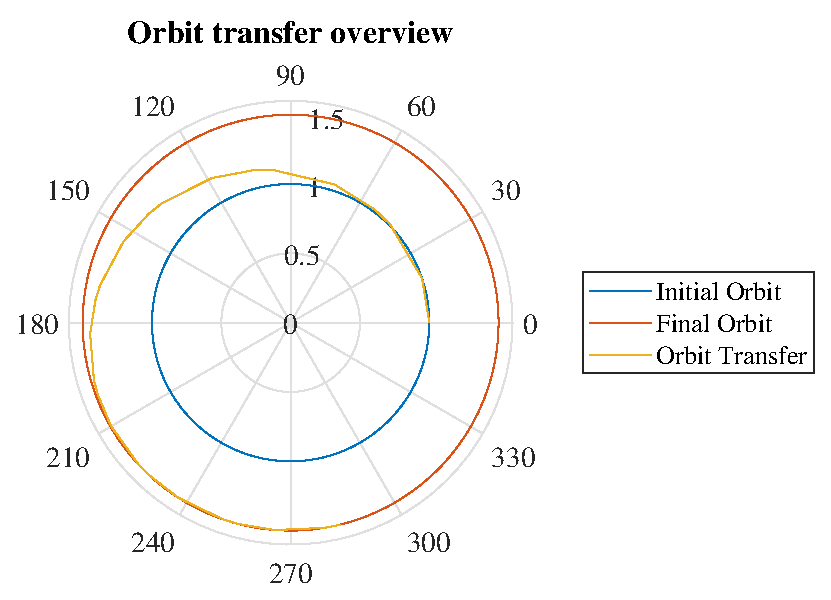
\includegraphics[scale=0.75]{orbit_N3_K8_C2_mf.eps}
	\caption{Trajectory from initial to final orbit (\(N:3\ , K:8\))}
	\label{fig:orbit_N3_K8_C2_mf}
\end{figure}
\begin{figure}
	\centering
	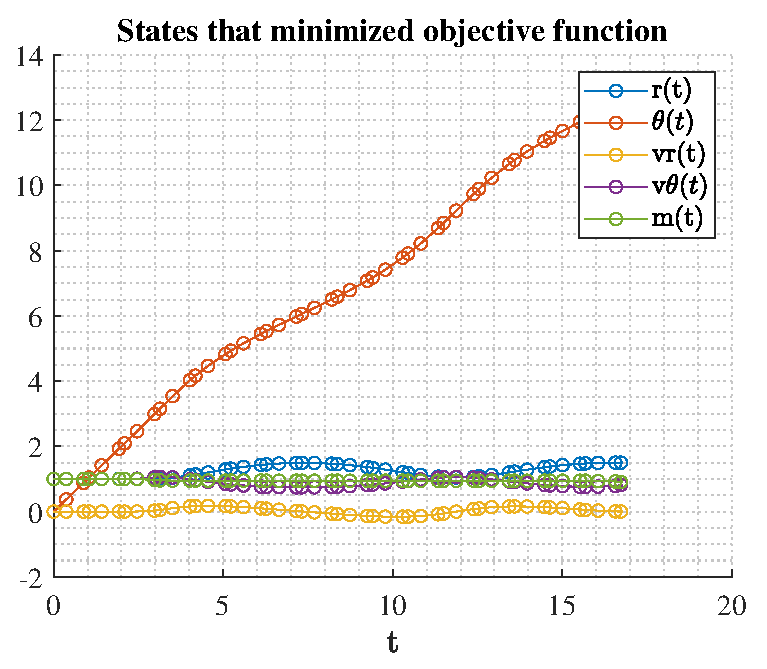
\includegraphics[scale=0.75]{states_N3_K16_C2_mf.eps}
	\caption{States for trajectory that maximized terminal mass (\(N:3\ , K:16\))}
	\label{fig:states_N3_K16_C2_mf}
\end{figure}
\begin{figure}
	\centering
	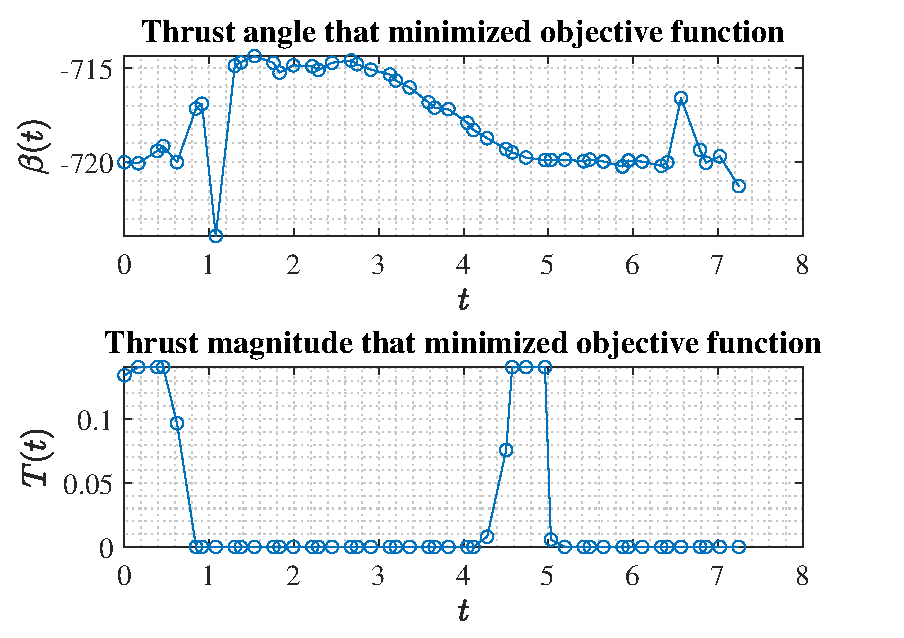
\includegraphics[scale=0.75]{control_N3_K16_C2_mf.eps}
	\caption{Control that maximized terminal mass (\(N:3\ , K:16\))}
	\label{fig:control_N3_K16_C2_mf}
\end{figure}
\begin{figure}
	\centering
	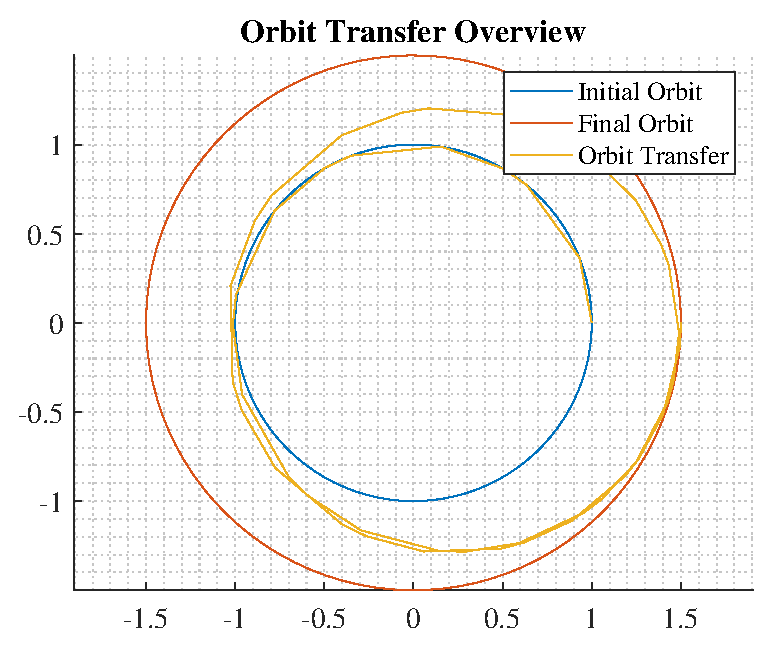
\includegraphics[scale=0.75]{orbit_N3_K16_C2_mf.eps}
	\caption{Trajectory from initial to final orbit (\(N:3\ , K:16\))}
	\label{fig:orbit_N3_K16_C2_mf}
\end{figure}
\begin{figure}
	\centering
	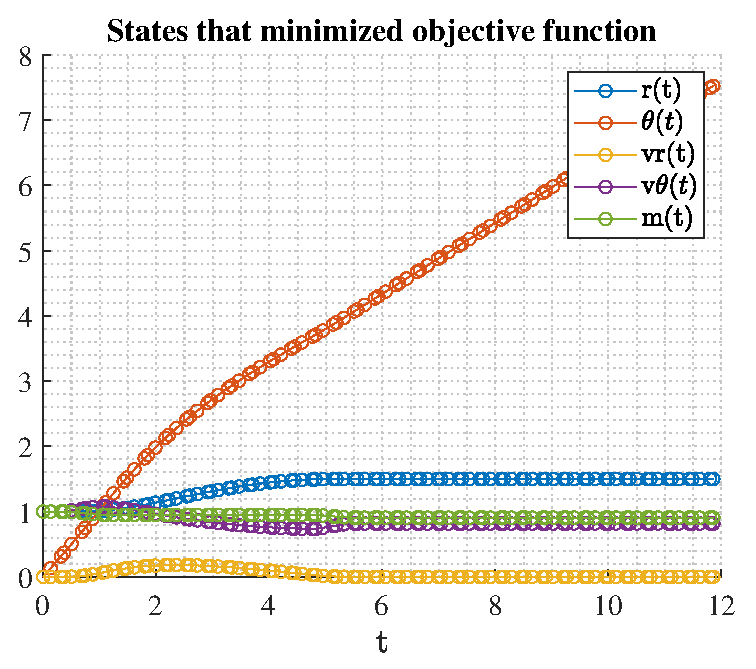
\includegraphics[scale=0.75]{states_N3_K32_C2_mf.eps}
	\caption{States for trajectory that maximized terminal mass (\(N:3\ , K:32\))}
	\label{fig:states_N3_K32_C2_mf}
\end{figure}
\begin{figure}
	\centering
	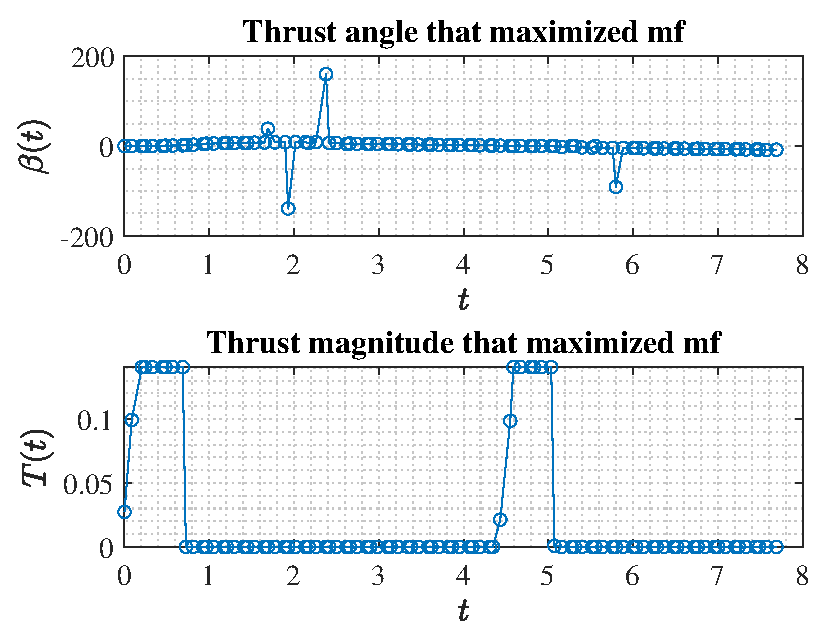
\includegraphics[scale=0.75]{control_N3_K32_C2_mf.eps}
	\caption{Control that maximized terminal mass (\(N:3\ , K:32\))}
	\label{fig:control_N3_K32_C2_mf}
\end{figure}
\begin{figure}
	\centering
	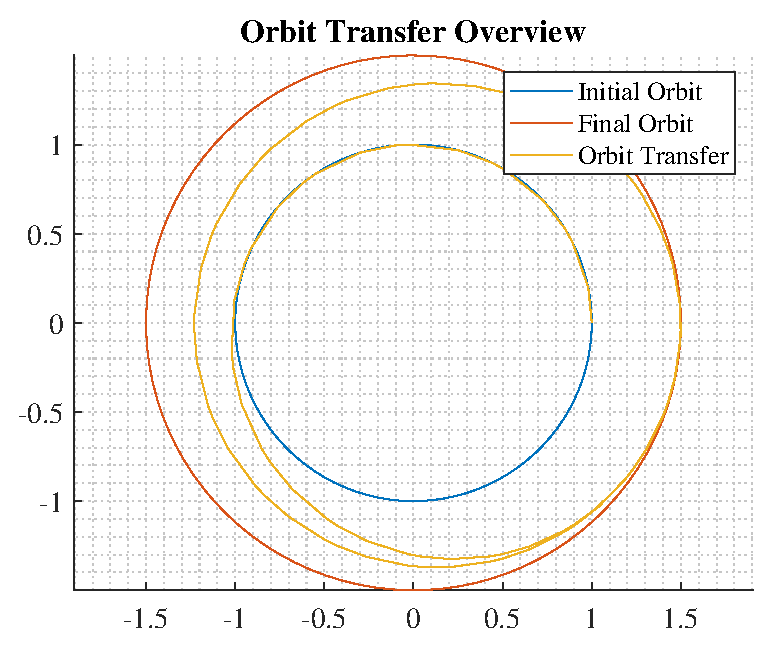
\includegraphics[scale=0.75]{orbit_N3_K32_C2_mf.eps}
	\caption{Trajectory from initial to final orbit (\(N:3\ , K:32\))}
	\label{fig:orbit_N3_K32_C2_mf}
\end{figure}
\begin{figure}
	\centering
	\includegraphics[scale=0.75]{states_N4_K2_C2_mf.eps}
	\caption{States for trajectory that maximized terminal mass (\(N:4\ , K:2\))}
	\label{fig:states_N4_K2_C2_mf}
\end{figure}
\begin{figure}
	\centering
	\includegraphics[scale=0.75]{control_N4_K2_C2_mf.eps}
	\caption{Control that maximized terminal mass (\(N:4\ , K:2\))}
	\label{fig:control_N4_K2_C2_mf}
\end{figure}
\begin{figure}
	\centering
	\includegraphics[scale=0.75]{orbit_N4_K2_C2_mf.eps}
	\caption{Trajectory from initial to final orbit (\(N:4\ , K:2\))}
	\label{fig:orbit_N4_K2_C2_mf}
\end{figure}
\begin{figure}
	\centering
	\includegraphics[scale=0.75]{states_N4_K4_C2_mf.eps}
	\caption{States for trajectory that maximized terminal mass (\(N:4\ , K:4\))}
	\label{fig:states_N4_K4_C2_mf}
\end{figure}
\begin{figure}
	\centering
	\includegraphics[scale=0.75]{control_N4_K4_C2_mf.eps}
	\caption{Control that maximized terminal mass (\(N:4\ , K:4\))}
	\label{fig:control_N4_K4_C2_mf}
\end{figure}
\begin{figure}
	\centering
	\includegraphics[scale=0.75]{orbit_N4_K4_C2_mf.eps}
	\caption{Trajectory from initial to final orbit (\(N:4\ , K:4\))}
	\label{fig:orbit_N4_K4_C2_mf}
\end{figure}
\begin{figure}
	\centering
	\includegraphics[scale=0.75]{states_N4_K8_C2_mf.eps}
	\caption{States for trajectory that maximized terminal mass (\(N:4\ , K:8\))}
	\label{fig:states_N4_K8_C2_mf}
\end{figure}
\begin{figure}
	\centering
	\includegraphics[scale=0.75]{control_N4_K8_C2_mf.eps}
	\caption{Control that maximized terminal mass (\(N:4\ , K:8\))}
	\label{fig:control_N4_K8_C2_mf}
\end{figure}
\begin{figure}
	\centering
	\includegraphics[scale=0.75]{orbit_N4_K8_C2_mf.eps}
	\caption{Trajectory from initial to final orbit (\(N:4\ , K:8\))}
	\label{fig:orbit_N4_K8_C2_mf}
\end{figure}
\begin{figure}
	\centering
	\includegraphics[scale=0.75]{states_N4_K16_C2_mf.eps}
	\caption{States for trajectory that maximized terminal mass (\(N:4\ , K:16\))}
	\label{fig:states_N4_K16_C2_mf}
\end{figure}
\begin{figure}
	\centering
	\includegraphics[scale=0.75]{control_N4_K16_C2_mf.eps}
	\caption{Control that maximized terminal mass (\(N:4\ , K:16\))}
	\label{fig:control_N4_K16_C2_mf}
\end{figure}
\begin{figure}
	\centering
	\includegraphics[scale=0.75]{orbit_N4_K16_C2_mf.eps}
	\caption{Trajectory from initial to final orbit (\(N:4\ , K:16\))}
	\label{fig:orbit_N4_K16_C2_mf}
\end{figure}
\begin{figure}
	\centering
	\includegraphics[scale=0.75]{states_N4_K32_C2_mf.eps}
	\caption{States for trajectory that maximized terminal mass (\(N:4\ , K:32\))}
	\label{fig:states_N4_K32_C2_mf}
\end{figure}
\begin{figure}
	\centering
	\includegraphics[scale=0.75]{control_N4_K32_C2_mf.eps}
	\caption{Control that maximized terminal mass (\(N:4\ , K:32\))}
	\label{fig:control_N4_K32_C2_mf}
\end{figure}
\begin{figure}
	\centering
	\includegraphics[scale=0.75]{orbit_N4_K32_C2_mf.eps}
	\caption{Trajectory from initial to final orbit (\(N:4\ , K:32\))}
	\label{fig:orbit_N4_K32_C2_mf}
\end{figure}
\begin{table}
	\begin{tabular}{lllllll}
		Degree & Intervals & Iterations & CPU Time & tf & mf & Solved\ Status \\ 
		\hline 
		3 & 2 & 621 & 1.96 & 10.5501 & 0.90956 & 0 \\ 
		3 & 4 & 4271 & 13.906 & 21.0208 & 0.90633 & -2 \\ 
		3 & 8 & 416 & 1.477 & 8.8194 & 0.90719 & 0 \\ 
		3 & 16 & 451 & 1.759 & 7.3181 & 0.9072 & 0 \\ 
		3 & 32 & 204 & 0.999 & 11.8567 & 0.9072 & 0 \\ 
		4 & 2 & 214 & 0.758 & 11.5211 & 0.90659 & -2 \\ 
		4 & 4 & 1720 & 5.772 & 7.6934 & 0.90717 & 0 \\ 
		4 & 8 & 231 & 0.903 & 9.4231 & 0.90718 & 0 \\ 
		4 & 16 & 138 & 0.657 & 10.3297 & 0.90721 & 0 \\ 
		4 & 32 & 131 & 0.749 & 8.2286 & 0.90719 & 1 \\ 
		\hline 
	\end{tabular}
	\caption{Results for maximizing \(m_f\) with unconstrained control}
	\label{table:2}
\end{table}
\FloatBarrier
	\subsection{Minimize Terminal Time with Constrained Control}
\begin{figure}
	\centering
	\includegraphics[scale=0.75]{states_N3_K2_C3_tf.eps}
	\caption{States for trajectory that minimized terminal time (\(N:3\ , K:2\))}
	\label{fig:states_N3_K2_C3_tf}
\end{figure}
\begin{figure}
	\centering
	\includegraphics[scale=0.75]{control_N3_K2_C3_tf.eps}
	\caption{Control that minimized terminal time (\(N:3\ , K:2\))}
	\label{fig:control_N3_K2_C3_tf}
\end{figure}
\begin{figure}
	\centering
	\includegraphics[scale=0.75]{path_N3_K2_C3_tf.eps}
	\caption{Path constrained control that minimized terminal time (\(N:3\ , K:2\))}
	\label{fig:path_N3_K2_C3_tf}
\end{figure}
\begin{figure}
	\centering
	\includegraphics[scale=0.75]{orbit_N3_K2_C3_tf.eps}
	\caption{Trajectory from initial to final orbit (\(N:3\ , K:2\))}
	\label{fig:orbit_N3_K2_C3_tf}
\end{figure}
\begin{figure}
	\centering
	\includegraphics[scale=0.75]{states_N3_K4_C3_tf.eps}
	\caption{States for trajectory that minimized terminal time (\(N:3\ , K:4\))}
	\label{fig:states_N3_K4_C3_tf}
\end{figure}
\begin{figure}
	\centering
	\includegraphics[scale=0.75]{control_N3_K4_C3_tf.eps}
	\caption{Control that minimized terminal time (\(N:3\ , K:4\))}
	\label{fig:control_N3_K4_C3_tf}
\end{figure}
\begin{figure}
	\centering
	\includegraphics[scale=0.75]{path_N3_K4_C3_tf.eps}
	\caption{Path constrained control that minimized terminal time (\(N:3\ , K:4\))}
	\label{fig:path_N3_K4_C3_tf}
\end{figure}
\begin{figure}
	\centering
	\includegraphics[scale=0.75]{orbit_N3_K4_C3_tf.eps}
	\caption{Trajectory from initial to final orbit (\(N:3\ , K:4\))}
	\label{fig:orbit_N3_K4_C3_tf}
\end{figure}
\begin{figure}
	\centering
	\includegraphics[scale=0.75]{states_N3_K8_C3_tf.eps}
	\caption{States for trajectory that minimized terminal time (\(N:3\ , K:8\))}
	\label{fig:states_N3_K8_C3_tf}
\end{figure}
\begin{figure}
	\centering
	\includegraphics[scale=0.75]{control_N3_K8_C3_tf.eps}
	\caption{Control that minimized terminal time (\(N:3\ , K:8\))}
	\label{fig:control_N3_K8_C3_tf}
\end{figure}
\begin{figure}
	\centering
	\includegraphics[scale=0.75]{path_N3_K8_C3_tf.eps}
	\caption{Path constrained control that minimized terminal time (\(N:3\ , K:8\))}
	\label{fig:path_N3_K8_C3_tf}
\end{figure}
\begin{figure}
	\centering
	\includegraphics[scale=0.75]{orbit_N3_K8_C3_tf.eps}
	\caption{Trajectory from initial to final orbit (\(N:3\ , K:8\))}
	\label{fig:orbit_N3_K8_C3_tf}
\end{figure}
\begin{figure}
	\centering
	\includegraphics[scale=0.75]{states_N3_K16_C3_tf.eps}
	\caption{States for trajectory that minimized terminal time (\(N:3\ , K:16\))}
	\label{fig:states_N3_K16_C3_tf}
\end{figure}
\begin{figure}
	\centering
	\includegraphics[scale=0.75]{control_N3_K16_C3_tf.eps}
	\caption{Control that minimized terminal time (\(N:3\ , K:16\))}
	\label{fig:control_N3_K16_C3_tf}
\end{figure}
\begin{figure}
	\centering
	\includegraphics[scale=0.75]{path_N3_K16_C3_tf.eps}
	\caption{Path constrained control that minimized terminal time (\(N:3\ , K:16\))}
	\label{fig:path_N3_K16_C3_tf}
\end{figure}
\begin{figure}
	\centering
	\includegraphics[scale=0.75]{orbit_N3_K16_C3_tf.eps}
	\caption{Trajectory from initial to final orbit (\(N:3\ , K:16\))}
	\label{fig:orbit_N3_K16_C3_tf}
\end{figure}
\begin{figure}
	\centering
	\includegraphics[scale=0.75]{states_N3_K32_C3_tf.eps}
	\caption{States for trajectory that minimized terminal time (\(N:3\ , K:32\))}
	\label{fig:states_N3_K32_C3_tf}
\end{figure}
\begin{figure}
	\centering
	\includegraphics[scale=0.75]{control_N3_K32_C3_tf.eps}
	\caption{Control that minimized terminal time (\(N:3\ , K:32\))}
	\label{fig:control_N3_K32_C3_tf}
\end{figure}
\begin{figure}
	\centering
	\includegraphics[scale=0.75]{path_N3_K32_C3_tf.eps}
	\caption{Path constrained control that minimized terminal time (\(N:3\ , K:32\))}
	\label{fig:path_N3_K32_C3_tf}
\end{figure}
\begin{figure}
	\centering
	\includegraphics[scale=0.75]{orbit_N3_K32_C3_tf.eps}
	\caption{Trajectory from initial to final orbit (\(N:3\ , K:32\))}
	\label{fig:orbit_N3_K32_C3_tf}
\end{figure}
\begin{figure}
	\centering
	\includegraphics[scale=0.75]{states_N4_K2_C3_tf.eps}
	\caption{States for trajectory that minimized terminal time (\(N:4\ , K:2\))}
	\label{fig:states_N4_K2_C3_tf}
\end{figure}
\begin{figure}
	\centering
	\includegraphics[scale=0.75]{control_N4_K2_C3_tf.eps}
	\caption{Control that minimized terminal time (\(N:4\ , K:2\))}
	\label{fig:control_N4_K2_C3_tf}
\end{figure}
\begin{figure}
	\centering
	\includegraphics[scale=0.75]{path_N4_K2_C3_tf.eps}
	\caption{Path constrained control that minimized terminal time (\(N:4\ , K:2\))}
	\label{fig:path_N4_K2_C3_tf}
\end{figure}
\begin{figure}
	\centering
	\includegraphics[scale=0.75]{orbit_N4_K2_C3_tf.eps}
	\caption{Trajectory from initial to final orbit (\(N:4\ , K:2\))}
	\label{fig:orbit_N4_K2_C3_tf}
\end{figure}
\begin{figure}
	\centering
	\includegraphics[scale=0.75]{states_N4_K4_C3_tf.eps}
	\caption{States for trajectory that minimized terminal time (\(N:4\ , K:4\))}
	\label{fig:states_N4_K4_C3_tf}
\end{figure}
\begin{figure}
	\centering
	\includegraphics[scale=0.75]{control_N4_K4_C3_tf.eps}
	\caption{Control that minimized terminal time (\(N:4\ , K:4\))}
	\label{fig:control_N4_K4_C3_tf}
\end{figure}
\begin{figure}
	\centering
	\includegraphics[scale=0.75]{path_N4_K4_C3_tf.eps}
	\caption{Path constrained control that minimized terminal time (\(N:4\ , K:4\))}
	\label{fig:path_N4_K4_C3_tf}
\end{figure}
\begin{figure}
	\centering
	\includegraphics[scale=0.75]{orbit_N4_K4_C3_tf.eps}
	\caption{Trajectory from initial to final orbit (\(N:4\ , K:4\))}
	\label{fig:orbit_N4_K4_C3_tf}
\end{figure}
\begin{figure}
	\centering
	\includegraphics[scale=0.75]{states_N4_K8_C3_tf.eps}
	\caption{States for trajectory that minimized terminal time (\(N:4\ , K:8\))}
	\label{fig:states_N4_K8_C3_tf}
\end{figure}
\begin{figure}
	\centering
	\includegraphics[scale=0.75]{control_N4_K8_C3_tf.eps}
	\caption{Control that minimized terminal time (\(N:4\ , K:8\))}
	\label{fig:control_N4_K8_C3_tf}
\end{figure}
\begin{figure}
	\centering
	\includegraphics[scale=0.75]{path_N4_K8_C3_tf.eps}
	\caption{Path constrained control that minimized terminal time (\(N:4\ , K:8\))}
	\label{fig:path_N4_K8_C3_tf}
\end{figure}
\begin{figure}
	\centering
	\includegraphics[scale=0.75]{orbit_N4_K8_C3_tf.eps}
	\caption{Trajectory from initial to final orbit (\(N:4\ , K:8\))}
	\label{fig:orbit_N4_K8_C3_tf}
\end{figure}
\begin{figure}
	\centering
	\includegraphics[scale=0.75]{states_N4_K16_C3_tf.eps}
	\caption{States for trajectory that minimized terminal time (\(N:4\ , K:16\))}
	\label{fig:states_N4_K16_C3_tf}
\end{figure}
\begin{figure}
	\centering
	\includegraphics[scale=0.75]{control_N4_K16_C3_tf.eps}
	\caption{Control that minimized terminal time (\(N:4\ , K:16\))}
	\label{fig:control_N4_K16_C3_tf}
\end{figure}
\begin{figure}
	\centering
	\includegraphics[scale=0.75]{path_N4_K16_C3_tf.eps}
	\caption{Path constrained control that minimized terminal time (\(N:4\ , K:16\))}
	\label{fig:path_N4_K16_C3_tf}
\end{figure}
\begin{figure}
	\centering
	\includegraphics[scale=0.75]{orbit_N4_K16_C3_tf.eps}
	\caption{Trajectory from initial to final orbit (\(N:4\ , K:16\))}
	\label{fig:orbit_N4_K16_C3_tf}
\end{figure}
\begin{figure}
	\centering
	\includegraphics[scale=0.75]{states_N4_K32_C3_tf.eps}
	\caption{States for trajectory that minimized terminal time (\(N:4\ , K:32\))}
	\label{fig:states_N4_K32_C3_tf}
\end{figure}
\begin{figure}
	\centering
	\includegraphics[scale=0.75]{control_N4_K32_C3_tf.eps}
	\caption{Control that minimized terminal time (\(N:4\ , K:32\))}
	\label{fig:control_N4_K32_C3_tf}
\end{figure}
\begin{figure}
	\centering
	\includegraphics[scale=0.75]{path_N4_K32_C3_tf.eps}
	\caption{Path constrained control that minimized terminal time (\(N:4\ , K:32\))}
	\label{fig:path_N4_K32_C3_tf}
\end{figure}
\begin{figure}
	\centering
	\includegraphics[scale=0.75]{orbit_N4_K32_C3_tf.eps}
	\caption{Trajectory from initial to final orbit (\(N:4\ , K:32\))}
	\label{fig:orbit_N4_K32_C3_tf}
\end{figure}
\begin{table}
	\begin{tabular}{lllllll}
		Degree & Intervals & Iterations & CPU Time & tf & mf & Solved\ Status \\ 
		\hline 
		3 & 2 & 47 & 0.225 & 3.2444 & 0.75569 & 0 \\ 
		3 & 4 & 69 & 0.446 & 3.2457 & 0.75559 & 0 \\ 
		3 & 8 & 77 & 0.369 & 3.2577 & 0.7581 & 0 \\ 
		3 & 16 & 119 & 0.537 & 3.247 & 0.7555 & 0 \\ 
		3 & 32 & 143 & 0.738 & 3.2623 & 0.75775 & 0 \\ 
		4 & 2 & 69 & 0.314 & 3.2456 & 0.7556 & 0 \\ 
		4 & 4 & 81 & 0.363 & 3.27 & 0.75761 & 0 \\ 
		4 & 8 & 102 & 0.464 & 3.2584 & 0.75655 & 0 \\ 
		4 & 16 & 143 & 0.677 & 3.247 & 0.7555 & 0 \\ 
		4 & 32 & 151 & 0.889 & 3.2482 & 0.75589 & 1 \\  
		\hline 
	\end{tabular}
	\caption{Results for minimizing \(t_f\) with constrained control}
	\label{table:3}
\end{table}
\FloatBarrier
	\subsection{Maximize Terminal Mass with Constrained Control}
\begin{figure}
	\centering
	\includegraphics[scale=0.75]{states_N3_K2_C3_mf.eps}
	\caption{States for trajectory that maximized terminal mass (\(N:3\ , K:2\))}
	\label{fig:states_N3_K2_C3_mf}
\end{figure}
\begin{figure}
	\centering
	\includegraphics[scale=0.75]{control_N3_K2_C3_mf.eps}
	\caption{Control that maximized terminal mass (\(N:3\ , K:2\))}
	\label{fig:control_N3_K2_C3_mf}
\end{figure}
\begin{figure}
	\centering
	\includegraphics[scale=0.75]{path_N3_K2_C3_mf.eps}
	\caption{Path constrained control that maximized terminal mass (\(N:3\ , K:2\))}
	\label{fig:path_N3_K2_C3_mf}
\end{figure}
\begin{figure}
	\centering
	\includegraphics[scale=0.75]{orbit_N3_K2_C3_mf.eps}
	\caption{Trajectory from initial to final orbit (\(N:3\ , K:2\))}
	\label{fig:orbit_N3_K2_C3_mf}
\end{figure}
\begin{figure}
	\centering
	\includegraphics[scale=0.75]{states_N3_K4_C3_mf.eps}
	\caption{States for trajectory that maximized terminal mass (\(N:3\ , K:4\))}
	\label{fig:states_N3_K4_C3_mf}
\end{figure}
\begin{figure}
	\centering
	\includegraphics[scale=0.75]{control_N3_K4_C3_mf.eps}
	\caption{Control that maximized terminal mass (\(N:3\ , K:4\))}
	\label{fig:control_N3_K4_C3_mf}
\end{figure}
\begin{figure}
	\centering
	\includegraphics[scale=0.75]{path_N3_K4_C3_mf.eps}
	\caption{Path constrained control that maximized terminal mass (\(N:3\ , K:4\))}
	\label{fig:path_N3_K4_C3_mf}
\end{figure}
\begin{figure}
	\centering
	\includegraphics[scale=0.75]{orbit_N3_K4_C3_mf.eps}
	\caption{Trajectory from initial to final orbit (\(N:3\ , K:4\))}
	\label{fig:orbit_N3_K4_C3_mf}
\end{figure}
\begin{figure}
	\centering
	\includegraphics[scale=0.75]{states_N3_K8_C3_mf.eps}
	\caption{States for trajectory that maximized terminal mass (\(N:3\ , K:8\))}
	\label{fig:states_N3_K8_C3_mf}
\end{figure}
\begin{figure}
	\centering
	\includegraphics[scale=0.75]{control_N3_K8_C3_mf.eps}
	\caption{Control that maximized terminal mass (\(N:3\ , K:8\))}
	\label{fig:control_N3_K8_C3_mf}
\end{figure}
\begin{figure}
	\centering
	\includegraphics[scale=0.75]{path_N3_K8_C3_mf.eps}
	\caption{Path constrained control that maximized terminal mass (\(N:3\ , K:8\))}
	\label{fig:path_N3_K8_C3_mf}
\end{figure}
\begin{figure}
	\centering
	\includegraphics[scale=0.75]{orbit_N3_K8_C3_mf.eps}
	\caption{Trajectory from initial to final orbit (\(N:3\ , K:8\))}
	\label{fig:orbit_N3_K8_C3_mf}
\end{figure}
\begin{figure}
	\centering
	\includegraphics[scale=0.75]{states_N3_K16_C3_mf.eps}
	\caption{States for trajectory that maximized terminal mass (\(N:3\ , K:16\))}
	\label{fig:states_N3_K16_C3_mf}
\end{figure}
\begin{figure}
	\centering
	\includegraphics[scale=0.75]{control_N3_K16_C3_mf.eps}
	\caption{Control that maximized terminal mass (\(N:3\ , K:16\))}
	\label{fig:control_N3_K16_C3_mf}
\end{figure}
\begin{figure}
	\centering
	\includegraphics[scale=0.75]{path_N3_K16_C3_mf.eps}
	\caption{Path constrained control that maximized terminal mass (\(N:3\ , K:16\))}
	\label{fig:path_N3_K16_C3_mf}
\end{figure}
\begin{figure}
	\centering
	\includegraphics[scale=0.75]{orbit_N3_K16_C3_mf.eps}
	\caption{Trajectory from initial to final orbit (\(N:3\ , K:16\))}
	\label{fig:orbit_N3_K16_C3_mf}
\end{figure}
\begin{figure}
	\centering
	\includegraphics[scale=0.75]{states_N3_K32_C3_mf.eps}
	\caption{States for trajectory that maximized terminal mass (\(N:3\ , K:32\))}
	\label{fig:states_N3_K32_C3_mf}
\end{figure}
\begin{figure}
	\centering
	\includegraphics[scale=0.75]{control_N3_K32_C3_mf.eps}
	\caption{Control that maximized terminal mass (\(N:3\ , K:32\))}
	\label{fig:control_N3_K32_C3_mf}
\end{figure}
\begin{figure}
	\centering
	\includegraphics[scale=0.75]{path_N3_K32_C3_mf.eps}
	\caption{Path constrained control that maximized terminal mass (\(N:3\ , K:32\))}
	\label{fig:path_N3_K32_C3_mf}
\end{figure}
\begin{figure}
	\centering
	\includegraphics[scale=0.75]{orbit_N3_K32_C3_mf.eps}
	\caption{Trajectory from initial to final orbit (\(N:3\ , K:32\))}
	\label{fig:orbit_N3_K32_C3_mf}
\end{figure}
\begin{figure}
	\centering
	\includegraphics[scale=0.75]{states_N4_K2_C3_mf.eps}
	\caption{States for trajectory that maximized terminal mass (\(N:4\ , K:2\))}
	\label{fig:states_N4_K2_C3_mf}
\end{figure}
\begin{figure}
	\centering
	\includegraphics[scale=0.75]{control_N4_K2_C3_mf.eps}
	\caption{Control that maximized terminal mass (\(N:4\ , K:2\))}
	\label{fig:control_N4_K2_C3_mf}
\end{figure}
\begin{figure}
	\centering
	\includegraphics[scale=0.75]{path_N4_K2_C3_mf.eps}
	\caption{Path constrained control that maximized terminal mass (\(N:4\ , K:2\))}
	\label{fig:path_N4_K2_C3_mf}
\end{figure}
\begin{figure}
	\centering
	\includegraphics[scale=0.75]{orbit_N4_K2_C3_mf.eps}
	\caption{Trajectory from initial to final orbit (\(N:4\ , K:2\))}
	\label{fig:orbit_N4_K2_C3_mf}
\end{figure}
\begin{figure}
	\centering
	\includegraphics[scale=0.75]{states_N4_K4_C3_mf.eps}
	\caption{States for trajectory that maximized terminal mass (\(N:4\ , K:4\))}
	\label{fig:states_N4_K4_C3_mf}
\end{figure}
\begin{figure}
	\centering
	\includegraphics[scale=0.75]{control_N4_K4_C3_mf.eps}
	\caption{Control that maximized terminal mass (\(N:4\ , K:4\))}
	\label{fig:control_N4_K4_C3_mf}
\end{figure}
\begin{figure}
	\centering
	\includegraphics[scale=0.75]{path_N4_K4_C3_mf.eps}
	\caption{Path constrained control that maximized terminal mass (\(N:4\ , K:4\))}
	\label{fig:path_N4_K4_C3_mf}
\end{figure}
\begin{figure}
	\centering
	\includegraphics[scale=0.75]{orbit_N4_K4_C3_mf.eps}
	\caption{Trajectory from initial to final orbit (\(N:4\ , K:4\))}
	\label{fig:orbit_N4_K4_C3_mf}
\end{figure}
\begin{figure}
	\centering
	\includegraphics[scale=0.75]{states_N4_K8_C3_mf.eps}
	\caption{States for trajectory that maximized terminal mass (\(N:4\ , K:8\))}
	\label{fig:states_N4_K8_C3_mf}
\end{figure}
\begin{figure}
	\centering
	\includegraphics[scale=0.75]{control_N4_K8_C3_mf.eps}
	\caption{Control that maximized terminal mass (\(N:4\ , K:8\))}
	\label{fig:control_N4_K8_C3_mf}
\end{figure}
\begin{figure}
	\centering
	\includegraphics[scale=0.75]{path_N4_K8_C3_mf.eps}
	\caption{Path constrained control that maximized terminal mass (\(N:4\ , K:8\))}
	\label{fig:path_N4_K8_C3_mf}
\end{figure}
\begin{figure}
	\centering
	\includegraphics[scale=0.75]{orbit_N4_K8_C3_mf.eps}
	\caption{Trajectory from initial to final orbit (\(N:4\ , K:8\))}
	\label{fig:orbit_N4_K8_C3_mf}
\end{figure}
\begin{figure}
	\centering
	\includegraphics[scale=0.75]{states_N4_K16_C3_mf.eps}
	\caption{States for trajectory that maximized terminal mass (\(N:4\ , K:16\))}
	\label{fig:states_N4_K16_C3_mf}
\end{figure}
\begin{figure}
	\centering
	\includegraphics[scale=0.75]{control_N4_K16_C3_mf.eps}
	\caption{Control that maximized terminal mass (\(N:4\ , K:16\))}
	\label{fig:control_N4_K16_C3_mf}
\end{figure}
\begin{figure}
	\centering
	\includegraphics[scale=0.75]{path_N4_K16_C3_mf.eps}
	\caption{Path constrained control that maximized terminal mass (\(N:4\ , K:16\))}
	\label{fig:path_N4_K16_C3_mf}
\end{figure}
\begin{figure}
	\centering
	\includegraphics[scale=0.75]{orbit_N4_K16_C3_mf.eps}
	\caption{Trajectory from initial to final orbit (\(N:4\ , K:16\))}
	\label{fig:orbit_N4_K16_C3_mf}
\end{figure}
\begin{figure}
	\centering
	\includegraphics[scale=0.75]{states_N4_K32_C3_mf.eps}
	\caption{States for trajectory that maximized terminal mass (\(N:4\ , K:32\))}
	\label{fig:states_N4_K32_C3_mf}
\end{figure}
\begin{figure}
	\centering
	\includegraphics[scale=0.75]{control_N4_K32_C3_mf.eps}
	\caption{Control that maximized terminal mass (\(N:4\ , K:32\))}
	\label{fig:control_N4_K32_C3_mf}
\end{figure}
\begin{figure}
	\centering
	\includegraphics[scale=0.75]{path_N4_K32_C3_mf.eps}
	\caption{Path constrained control that maximized terminal mass (\(N:4\ , K:32\))}
	\label{fig:path_N4_K32_C3_mf}
\end{figure}
\begin{figure}
	\centering
	\includegraphics[scale=0.75]{orbit_N4_K32_C3_mf.eps}
	\caption{Trajectory from initial to final orbit (\(N:4\ , K:32\))}
	\label{fig:orbit_N4_K32_C3_mf}
\end{figure}
\begin{table}
	\begin{tabular}{lllllll}
		Degree & Intervals & Iterations & CPU Time & tf & mf & Solved\ Status \\ 
		\hline 
		3 & 2 & 110 & 0.417 & 15.0512 & 0.90547 & -2 \\ 
		3 & 4 & 2185 & 7.269 & 14.4119 & 0.9095 & 0 \\ 
		3 & 8 & 728 & 2.557 & 6.9851 & 0.90719 & 0 \\ 
		3 & 16 & 96 & 0.465 & 7.9129 & 0.9072 & 0 \\ 
		3 & 32 & 102 & 0.559 & 6.689 & 0.90721 & 1 \\ 
		4 & 2 & 531 & 1.765 & 12.3575 & 0.91207 & 0 \\ 
		4 & 4 & 415 & 1.465 & 6.1534 & 0.90718 & 0 \\ 
		4 & 8 & 397 & 1.511 & 7.0005 & 0.90721 & 0 \\ 
		4 & 16 & 141 & 0.688 & 6.3843 & 0.90721 & 1 \\ 
		4 & 32 & 1016 & 5.404 & 7.0926 & 0.90721 & 1 \\ 
		\hline 
	\end{tabular}
	\caption{Results for maximizing \(m_f\) with constrained control}
	\label{table:4}
\end{table}
\FloatBarrier

	\subsection{Overall Analysis}
	
	\section{Future Work}

	
	\section{Appendix}
	\lstinputlisting[label=orbitTransferMain,    caption = orbitTransferMain.m]{../orbitTransferMain.m}
	\lstinputlisting[label=orbitTransferFun,     caption = orbitTransferFun.m]{../orbitTransferFun.m}
	\lstinputlisting[label=orbitTransferObj,     caption = orbitTransferObj.m]{../orbitTransferObj.m}
	\lstinputlisting[label=orbitTransferCon,     caption = orbitTransferCon.m]{../orbitTransferCon.m}
	\lstinputlisting[label= orbitTransferGrd,    caption = orbitTransferGrd.m]{../orbitTransferGrd.m}
	\lstinputlisting[label= orbitTransferJac,    caption = orbitTransferJac.m]{../orbitTransferJac.m}
    \lstinputlisting[label= orbitTransferJacPat, caption = orbitTransferJacPat.m]{../orbitTransferJacPat.m}
\end{document}
